% 美赛模板:正文部分

\documentclass[12pt]{article}  % 官方要求字号不小于 12 号,此处选择 12 号字体
% \linespread{1.1}
% \bibliographystyle{plain}
% 本模板不需要填写年份,以当前电脑时间自动生成
% 请在以下的方括号中填写队伍控制号
\usepackage[2006782]{easymcm}  % 载入 EasyMCM 模板文件
\problem{D}  % 请在此处填写题号
% \usepackage{mathptmx}  % 这是 Times 字体,中规中矩 
\usepackage{palatino}  % mathpazo 这palatino是 COMAP 官方杂志采用的更好看的 Palatino 字体,可替代以上的 mathptmx 宏包
\usepackage{pdfpages}
\usepackage{longtable}
\usepackage{tabu}
\usepackage{threeparttable}
\usepackage{listings}
\usepackage{paralist}
 \let\itemize\compactitem
 \let\enditemize\endcompactitem
% \let\enumerate\compactenum
% \let\endenumerate\endcompactenum
% \let\description\compactdesc
% \let\enddescription\endcompactdesc
% \usepackage{biblatex} 
% \usepackage{cite}
% \usepackage{natbib}
\newcommand{\upcite}[1]{\textsuperscript{\textsuperscript{\cite{#1}}}}
\title{Teaming Wisdom Coming from Soccer Field}  % 标题

% 如需要修改题头(默认为 MCM/ICM),请使用以下命令(此处修改为 MCM)
%\renewcommand{\contest}{MCM}

% 文档开始
\begin{document}

% 此处填写摘要内容
\begin{abstract}
    
    % (Need to be reviewed)
    Nowadays teamwork is playing an increasingly important role in all walks of life, especially team sports. Team success is much more than the sum of the abilities of individual players. Rather, it is based on many other factors that involve how well the teammates play together. The purpose of this paper is to create a model that captures performance indicators that reflect successful teamwork, and generalize the model to other domains.

In \textsc{Task 1}, we establish a \textit{ball passing network} based on the passing events, in which each player is a node and each pass constitutes a link between players. We define several indicators helping us know about the network on the whole. Then we utilize \textit{K-means Algorithm} to classify \textit{dyadic and triadic configurations} in the network, which help to identify the network patterns. Moreover, we explore the network with other scales like time and region to further study the network.

In \textsc{Task 2}, we first identify performance indicators that reflect successful teamwork, such as coordination, distribution, tempo, flexibility and pressing. Then an \textit{Evaluation model based on Adversarial Regression} is built to score the teamwork performance of both our team and opponent in one match. To make scores of both teams satisfy the final result of each game, we regulate the weights of five indicators, and record every possible solution. Furthermore, we choose the weight with $\mathtt{LowestError}$ as the regression equation. Finally,  we notice that only by adjusting the strategy based on the opponents' strategy, trying to make the total score higher or repress the score of opponents, can the Huskies more likely to win.

In \textsc{Task 3}, we analyze the formations and strategies Huskies adopt, along with the indicators and final results. Considering the actual situation of the Huskies, the most effective strategy is \textit{Defensive counterattack}. Then comparing Huskies with Typical representative of this strategy (\textit{Italy National Team}), we get to know that the huge gap with the strong teams is mainly reflected in \textit{Coordination}, \textit{Flexibility} and \textit{Pressing}. Based on the conclusion we draw, we offer the coach some advice on \textit{flexible formation}, \textit{core players} and \textit{coherence} that help them succeed in the next season. 

In \textsc{Task 4}, we generalize our model to more teamwork, not limited to team sports. With reference to the indicators we identify for football match, we come up with the complex set of factors that make some groups perform better. In addition, other aspects of teamwork are taken into account to organize more effective teams.

Finally, we conduct a sensitivity analysis in order to gain some deep understanding of our model, and verify the robustness of the model in many cases. Additionally, we analyze the strengths and weaknesses of our model.


    

    % Here is the abstract of your paper.

    % Firstly, that is ...

    % Secondly, that is ...

    % Finally, that is ...

    % 美赛论文中无需注明关键字。若您一定要使用,
    % 请将以下两行的注释号 '%' 去除,以使其生效
    \vspace{5pt}
    \textbf{Keywords}: Passing network, Adversarial Regression, Defensive Counterattack

\end{abstract}

\maketitle  % 生成 Summary Sheet

\tableofcontents  % 生成目录


% 正文开始
% Chapter 1: Introduction
\section{Introduction}

\subsection{Problem Background}
With the development of social interconnections, the challenge people faced has become complex increasingly. Some reports point out the best strategies for team formation, the best interaction between teammates, and the ideal leadership style. A strong team across departments and domains can complete complex tasks that cannot be accomplished through individual efforts or additional contributions from a series of teammates.

The coach has asked ICM to quantify and formalize the structural and dynamical features that have been successful (and unsuccessful) for the team. The team are provided with the following tasks:
\begin{itemize}
    \setlength{\parsep}{0ex} %段落间距
    \setlength{\topsep}{2ex} %列表到上下文的垂直距离
    \setlength{\itemsep}{1ex} %条目间距
    \item Create a network for the ball passing between players, and explore multiple scales such as regions and time.
    \item Identify performance indicators that reflect successful teamwork.
    \item Make suggestions to the coach using the opinions gained from the model.
    \item Indicate how to build an effective team and give other important factors for forming an dynamic team.
\end{itemize}



\subsection{Our work}

\begin{enumerate}[\bfseries 1.]
    \setlength{\parsep}{0ex} %段落间距
    \setlength{\topsep}{2ex} %列表到上下文的垂直距离
    \setlength{\itemsep}{1ex} %条目间距
    \item Firstly, we establish a \textit{ball passing network} based on the passing events.Then we utilize \textit{K-means agAlgorithmm} to classify dyadic and triadic configurations in the network.
    \item Then we build an \textit{Evaluation model based on Adversarial Regression}, and get the regression equation.  Taking the opponents into account, we have a discussion about whether strategies are universally effective.
    \item Furthermore, We analyze the formations and strategies Huskies adopt and recommend the team to adopt \textit{Defensive counterattack}. What's more, we get to know the gap with strong team after comparing with \textit{Italy National Team}.
    \item Last but not least, we generalize our model to more teamwork and indicate how to build an effective team and give other important factors for forming an dynamic team.
\end{enumerate}



% \section{Introduction}
% \subsection{Problem Background}
% Here is the problem background ...

% Two major problems are discussed in this paper, which are:
% \begin{itemize}
%     \item Doing the first thing.
%     \item Doing the second thing.
% \end{itemize}

% \subsection{Literature Review}
% A literatrue\cite{1} say something about this problem ...

% \subsection{Our work}
% We do such things ...

% \begin{enumerate}[\bfseries 1.]
%     \item We do ...
%     \item We do ...
%     \item We do ...
% \end{enumerate}

% Chapter 2: 模型准备
\section{Preparation of the Models}
\subsection{Assumptions and Justifications}
\begin{itemize}
    \setlength{\parsep}{0ex} %段落间距
    \setlength{\topsep}{2ex} %列表到上下文的垂直距离
    \setlength{\itemsep}{1ex} %条目间距
    \item The ball passing network is an undirected graph.
    \item The incoming player substitutes the outgoing player directly, without changing the team formation. 
    \item There is no difference between the opponents' strength level, which lies in the opponents' counter strategy. 
    \item Each player, either of Huskies or of opponents, has the same physical quality and individual ability.  
\end{itemize}


\subsection{Notations}
The primary notations used in this paper are listed in Table \ref{tb:notation}.
\begin{table}[!htbp]
\begin{center}
\caption{Notations}
\begin{tabular}{c|l}
	\toprule
	\multicolumn{1}{m{3cm}}{\centering Symbol}
	&\multicolumn{1}{m{8cm}}{\centering Definition}\\
	\midrule
    $L$& Total links of network \\
    $\rho$& Network Density \\
    $w_{ij}$& Number of passes\\
    $d_{ij}$& topological distance \\
    $D$ & Network Diameter \\
    $C(i)$& Clustering Coefficient\\
    $f$ & ratio of goals to shots\\
    $d$ & ratio of defenses to losses\\
    $\varphi$& Distribution of contributes\\
    $t_b$&50-ball Passing Time\\
    $\mu_i$& Number of shots\\
    $\nu_i$& Number of defenses\\    
    $S$ & Score of teamwork\\
    $\beta_i$ & Weight of indicators \\
    $\gamma$& Coordination among players\\
    \bottomrule
\end{tabular}\label{tb:notation}
\end{center}
\end{table}


% % Chapter 3:其他假设
% \section{Assumptions and Justifications}
% First and foremost, we make some basic assumptions about dragons and explain their rationales.
% \begin{enumerate}[\bfseries \text{Assumption} 1 ]
%     \item \textit{They continue to grow throughout their life depending on the conditions and amount of food available to them.} 
%     \item \textit{Dragons are able to fly great distances, breath fire.}
%     \item \textit{During the time scale we discuss in this paper, the earth's ecological environment keeps stable.}
    
%     In our model, we don't consider the incidents that may cause great climate changes such as meteorite impacts or frequent volcanoes, since their probabilities are small.
%     \item \textit{During the time scale we discuss in this paper, a dragon's body function won't change as the dragon grows old.}
    
%     \item \textit{Dragons are at the top of the food chain.}
    
%     Considering the power of dragons, the dragons can have influence on all living beings in the ecosystem while few living beings can compete with the dragon.
%     \item \textit{Dragon's body function won't change when it is hurt.}
    
%     Dragons can resist tremendous trauma.
%     \item \textit{There is a upper bound for dragon's body size.}
    
%        With the limitation of gravity and biological structure, the body size of a dragon cannot     infinitely increase.
 
% \end{enumerate}

% Then, we will make some useful assumptions in the tasks to perfect the problems.
% \begin{enumerate}[\bfseries 1.]
% \item The living area of the dragon is related to the quantity, intimacy, and the average weight of the dragon.
% \item the growth rate parameter of the dragon
% increases with the increase of the weight of the food.
% \item Dragon survives in an ideal environment and is not affected by human activities.
% \item Dragon's body state is similar to that of flying
% creatures.
% \end{enumerate}

% Below, we next explore dragon characteristics, behavior, habits, diet, and interaction with their environment. Based on the additional assumptions mentioned above, four major tasks have yet to be addressed (see \textbf{Figure \ref{fig:tasks}}).

% \clearpage
\section{\textsc{Task 1: }Ball Passing Network Model}
\subsection{Construction of Ball Passing Network}
\subsubsection{Ball Passing Network}
Considering the relationship between players on the football field, the network for the ball passing can be described as an \textit{adjacency matrix}\upcite{1} in Data Structure. An adjacency matrix can be generated to perform network analysis, which represents the connections between a node (player) and an adjacency node (teammate). To generate an adjacency matrix for network analysis, you must define criteria that characterize the connections. We define $w_{ij}$ as the number of passes between player $i$ and player $j$. The adjacency matrix between players can be expressed as:

\begin{equation}\label{Eq:matrix1}
    \bordermatrix{%
           & \scriptstyle 1       & \scriptstyle 2     &\scriptstyle \cdots     &\scriptstyle 11\cr
    \scriptstyle 1    & w_{11}         & w_{12}       &\cdots     & w_{1,11}\cr
    \scriptstyle 2    & w_{21}         & w_{21}       &\cdots     & w_{2,11}\cr
    \scriptstyle\vdots & \vdots    &\vdots   &\cdots     &\vdots\cr
    \scriptstyle 11    & w_{11,1}         & w_{11,2}       &\cdots     &w_{11,11}
    },
    \end{equation}
In this paper, we assume that the ball passing network is an \textit{undirected graph}, which means the edge has no direction. Therefore, we have the number of passes between players $w_{ij}=w_{ji}$

Meanwhile, the ball passing network can be vividly illustrated in \textbf{Figure \ref{fig:exam_network}} by \textit{Gephi}.
\begin{figure}[htbp]
    \centering
    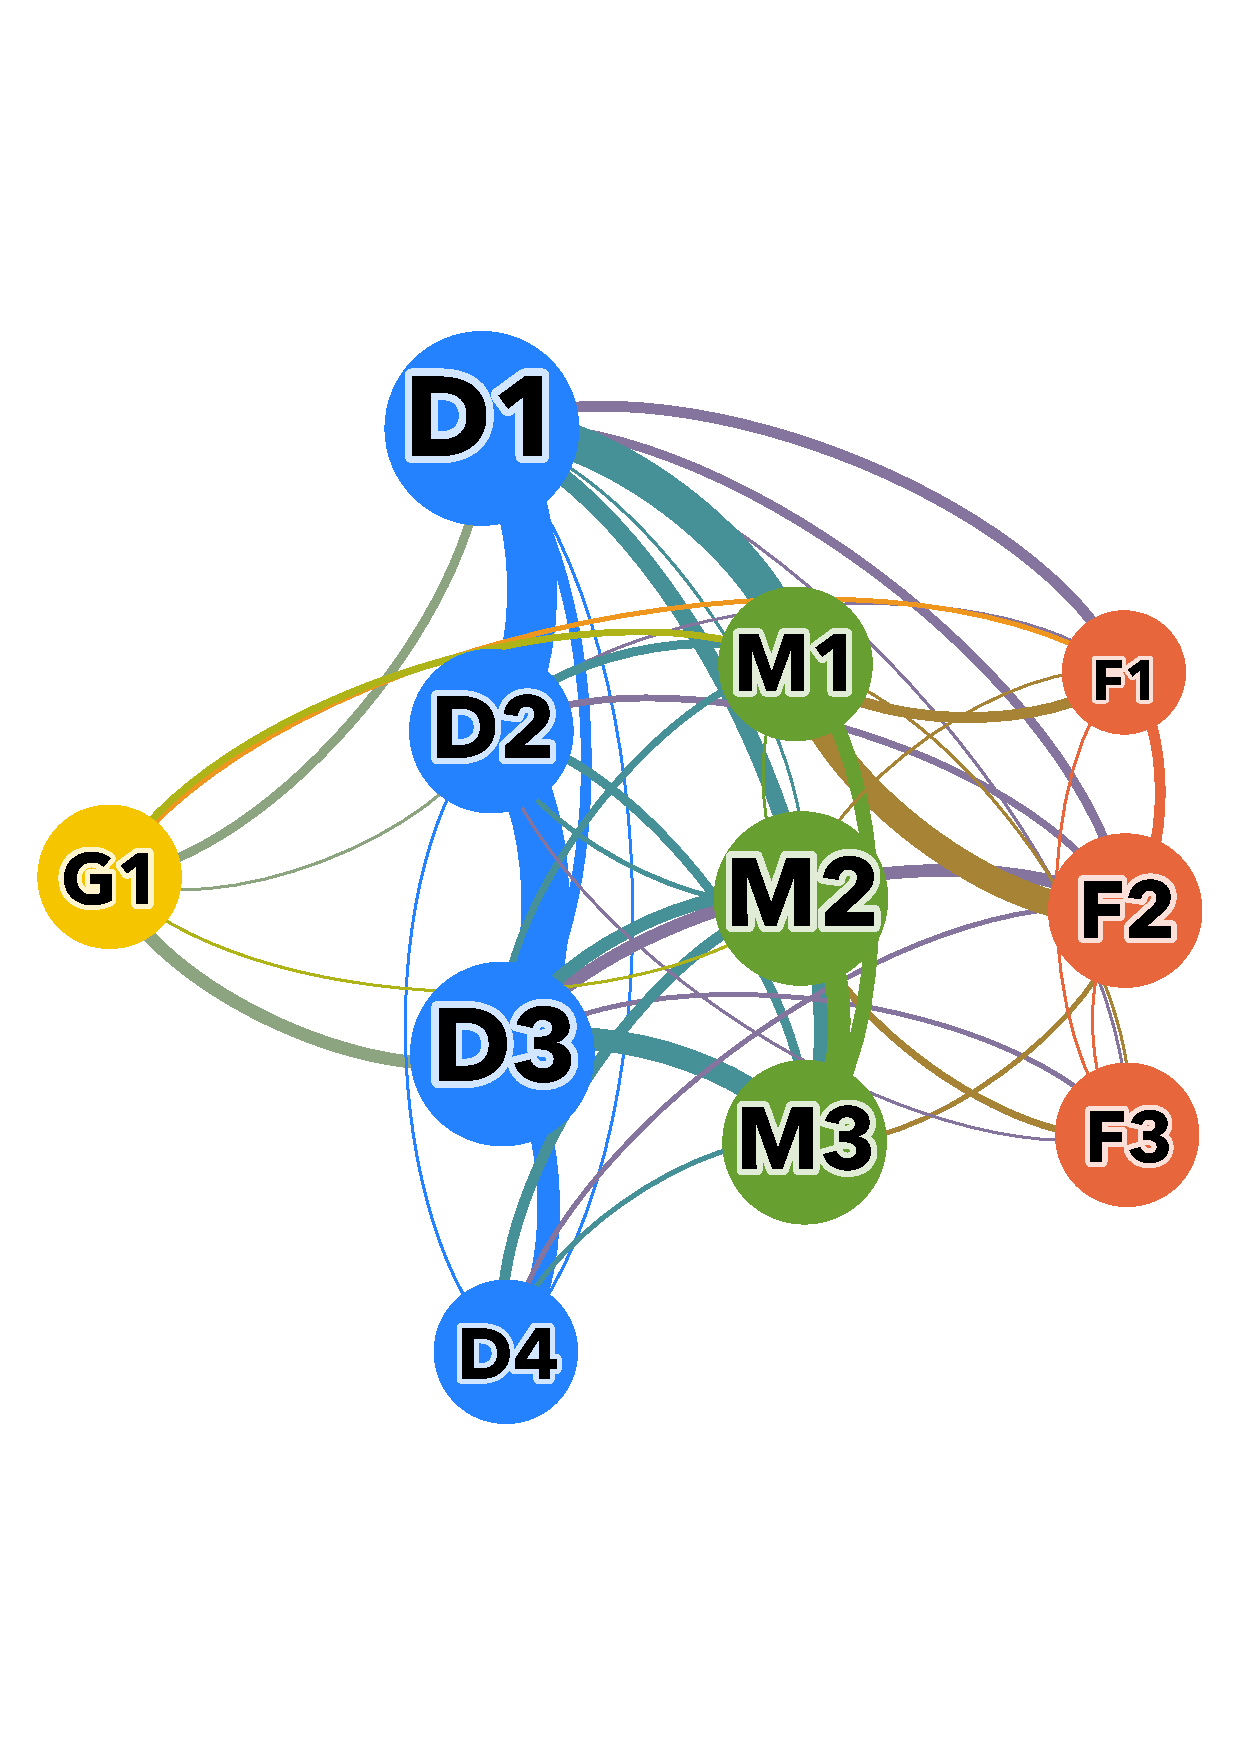
\includegraphics[width=.35\textwidth]{matrix_describe.pdf} 	% 图片相对位置
    \caption{An example of the ball passing network}		% 图片标题 
    \label{fig:exam_network}							% 图片标签
\end{figure}

Where width of the links are proportional to their weights, while the size of the nodes correspond to the number of passes.


\subsubsection{Determination of Network Parameter}
In order to further understand the network model, we should select some relevant indicators. The ball passing network analysis of the Huskies was focused on the following four measures based on the connections between teammates: \textit{total links}, \textit{density}, \textit{diameter}, and \textit{clustering coefficient}.

\vspace{4pt}
\begin{itemize}
    \item \textbf{Total Links $L$}
\end{itemize}

The sum of the elements of each row of the adjacency matrix $\sum_{j=1}^{11}$ is the total number of passes between player $i$ and all other teammates, which is the \textit{degree} in \textit{Graph Theory}. A node with a higher degree is a player who made more considerable passes with most of its teammates. This shows that the player is involved in the attacking development of his team..

In an undirected graph, the \textit{Total Links} ($L$) between each team player is a significant parameter in the analysis, which the value is half of the total sum of each adjacency matrix row sum.
\begin{equation}\label{eq:total_links}
    L=\frac{1}{2} \sum_{j=1}^{11} \sum_{i=1}^{11} w_{ij}.
\end{equation}

The \textit{Total Links} is very useful when evaluating the performance of a team, as it is the absolute number of total interactions between teammates in a match. Therefore, the team's average total link index is higher than the average, which indicates a strong cooperation among team members. 

\vspace{4pt}
\begin{itemize}
    \item \textbf{Network Density} $\rho$
\end{itemize}

\textit{Total Links} is the number of absolute interactions between one player and another player. However, the \textit{Network Density} of team is a relative parameter, and it can also measure the overall emotion between teammates.\upcite{2}

In graph theory, the density of a graph is proportional to the maximum number of possible adjacency edges. Let's consider the number of edges in the graph as $n$. Thus, the \textit{Network Density} $\rho$ is defined as the ratio of the \textit{Total Links} $L$ to the maximum number of possible adjacency edges as follow:
\begin{equation}\label{eq:network_density}
    \rho=\frac{L}{\mathbf{C}_n^2},
\end{equation}
where in this paper the number of edges $n=11$, so the density $\rho=\frac{L}{55}$.

\vspace{4pt}
\begin{itemize}
    \item \textbf{Network Diameter} $D$
\end{itemize}

The \textit{Network Diameter} $D$ of a network reflects how far, at most, two nodes in the graph are. 
The topological distance $d_{ij}$ of the link between two players $i$ and $j$ is defined as the inverse of the link weight. 
\begin{equation}\label{eq:topological_distance}
    d_{ij}=\frac{1}{w_{ij}}
\end{equation}
The \textit{Diameter} $D$ of a graph is the maximum topological distance\upcite{3} (the length of the largest geodesic) between any two players and can be expressed as:
\begin{equation}
    D=\max_i\max_j d_{ij}.
\end{equation}

In case of team players, a small diameter reflects a low maximum distance between teammates, which may reveal that the team's passing game was diffused among most of its players (rather than a few acting as central ones).

\vspace{4pt}
\begin{itemize}
    \item \textbf{Clustering coefficient} $C(i)$
\end{itemize}

Considering the network is weighted, we can not simply account for the number of nodes connected between them but how the link weights are distributed. In the case of the \textit{ball passing network}, the number of passes between pairs of players is not constant. As a consequence, we use a \textit{Weighted Clustering Coefficient}\upcite{4} $C_w(i)$ to measure the possibility that a given player $i$'s teammates will also create a connection between them:
\begin{equation}
    C_w(i)=\frac{\displaystyle\sum_{j}\sum_{k}w_{ij}w_{jk}w_{ik}}{\displaystyle\sum_{j}\sum_{k}w_{ij}w_{ik}}.
\end{equation}
Where $j$ and $k$ are the two teammates of player $i$, $w_{ij}$ and $w_{ik}$ are the number of ball passes between player $i$ and both them.
At last, the \textit{Clustering Coefficient} $C_i$ for the entire network is obtained by averaging $C_w(i)$ for all players, i.e.
\begin{equation}
    C=\frac{1}{n}\sum_{i=1}^{n} C_w(i),
\end{equation}
where in this paper the number of edges $n=11$.

\subsection{Identification of Network Patterns}
\subsubsection{Team Formation}
The formation of each game can be easily obtained by looking through the player list. In the dataset provided for us, all players are placed in four positions, which are \textit{goalkeeper}, \textit{defense}, \textit{midfield} and \textit{forward}. So when we study the formation in one game, we place the players in the position his ID indicates, thus obtaining the formation. To simplify the model, we assume that the substituted player replaces the player substituted directly, without changing the formation. 
We take the 1\textsuperscript{st}, the 2\textsuperscript{nd} and the 4\textsuperscript{th} match as examples. 
The formation of these matches means a teamwork strategy. Take \textsf{4-3-3} as an example, this formation means we have 4 defenses , 3 midfields and 3 forwards.
% The formation of these matches can be vividly illustrated by \textbf{Figure \ref{fig:task1_formation}}.

% \begin{figure}[htbp]
%     \centering
%     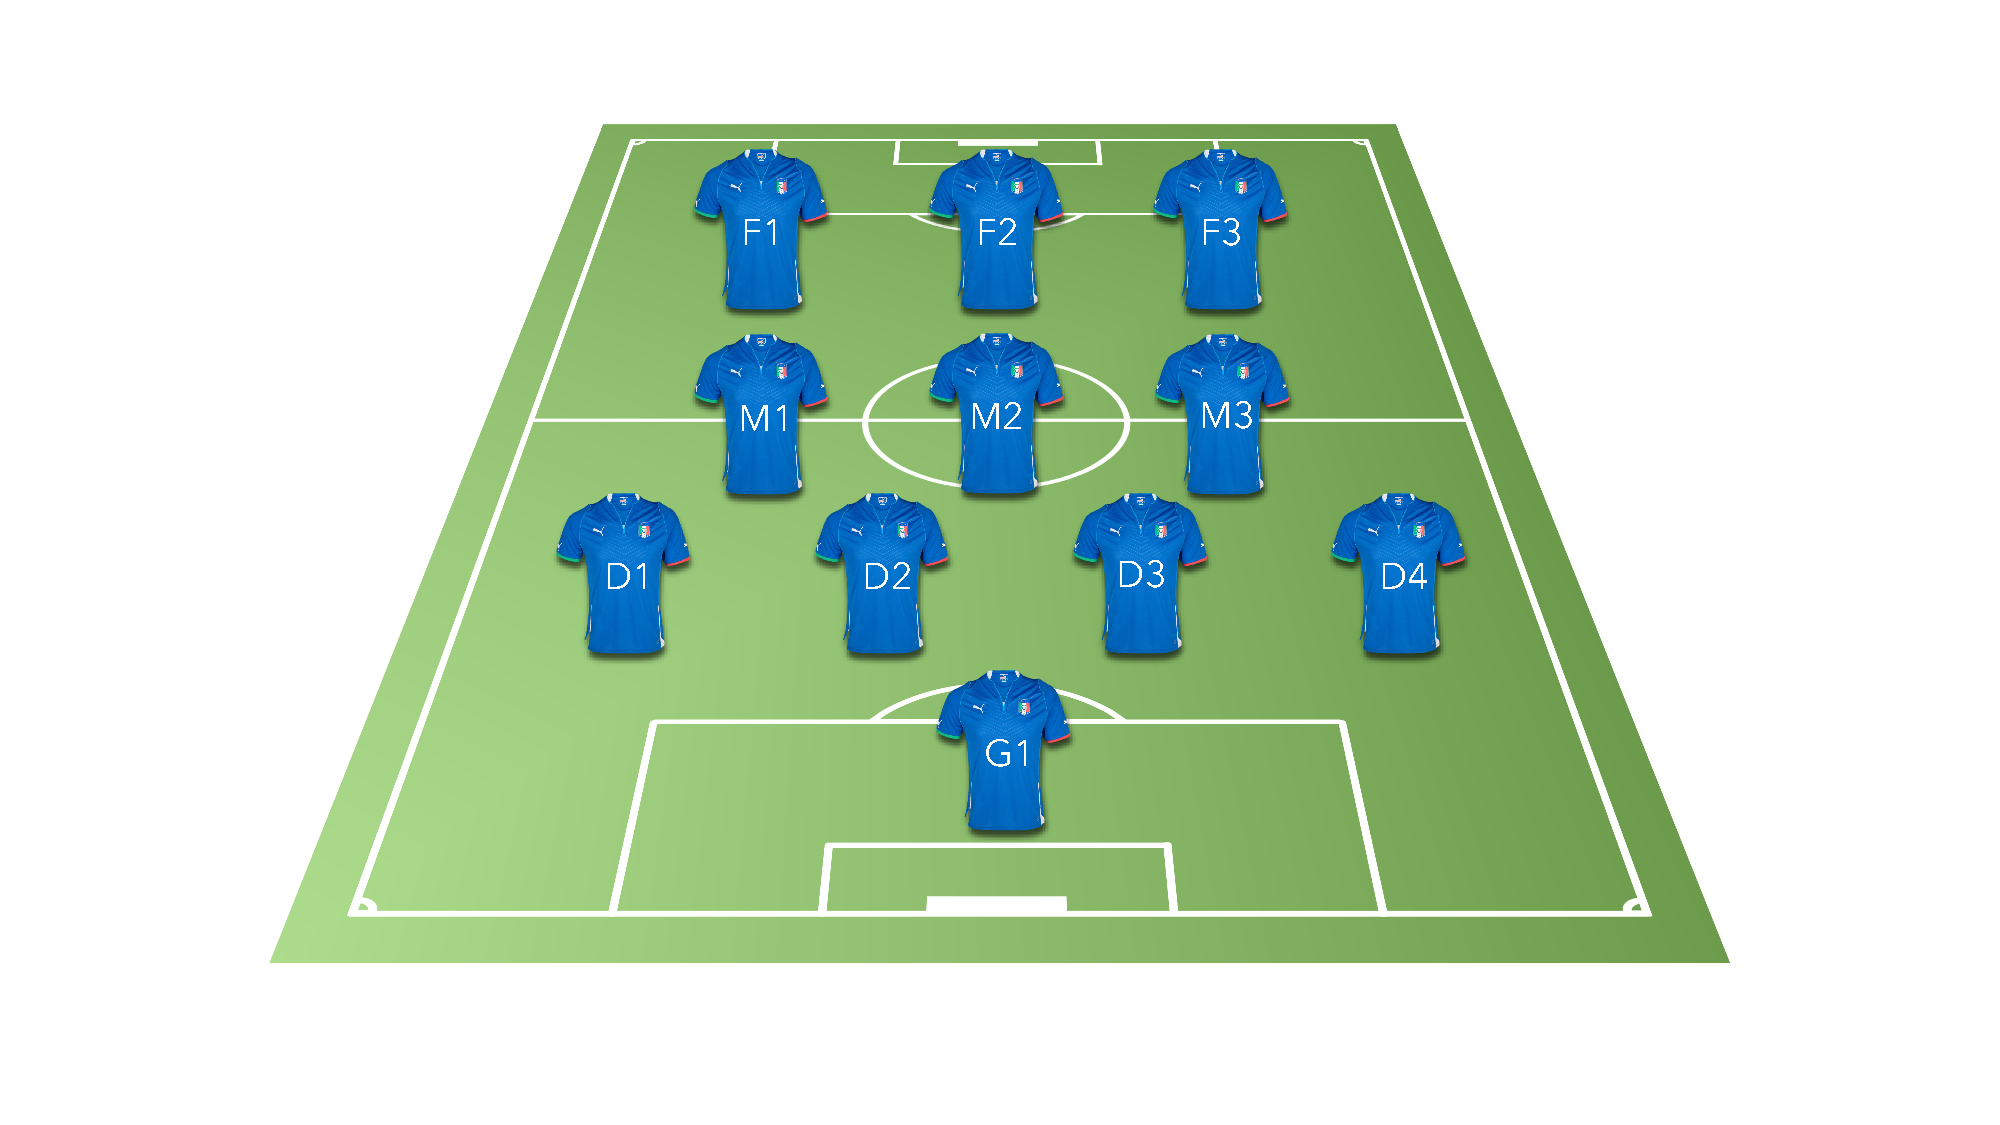
\includegraphics[width=.65\textwidth]{task1_formation.pdf} 	% 图片相对位置
%     \caption{An example of Team Formation}		% 图片标题 
%     \label{fig:task1_formation}							% 图片标签
% \end{figure}

The 1\textsuperscript{st} match Huskies take \textsf{4-3-3} formation, while the formations of the 2\textsuperscript{nd} and the 4\textsuperscript{th} matches are \textsf{5-3-2} and \textsf{4-4-2} respectively. In each game, the coach will take different formations according to the strategy, so figuring out the formation is important to understand the strategy, thus better identifying the network pattern. However, formation just gives us a general view of the network. To identify the network pattern more comprehensively, we need more details of the network. 

\subsubsection{Dyadic and Triadic Configurations}
Considering the difference in opponent and strategy, the ball passing network we build varies from match to match. Therefore, in order to identify the network pattern, we need to analyze a specific game in detail. In this chapter, we take the 1\textsuperscript{st} match as an example.

\begin{figure}[htbp]
    \centering
    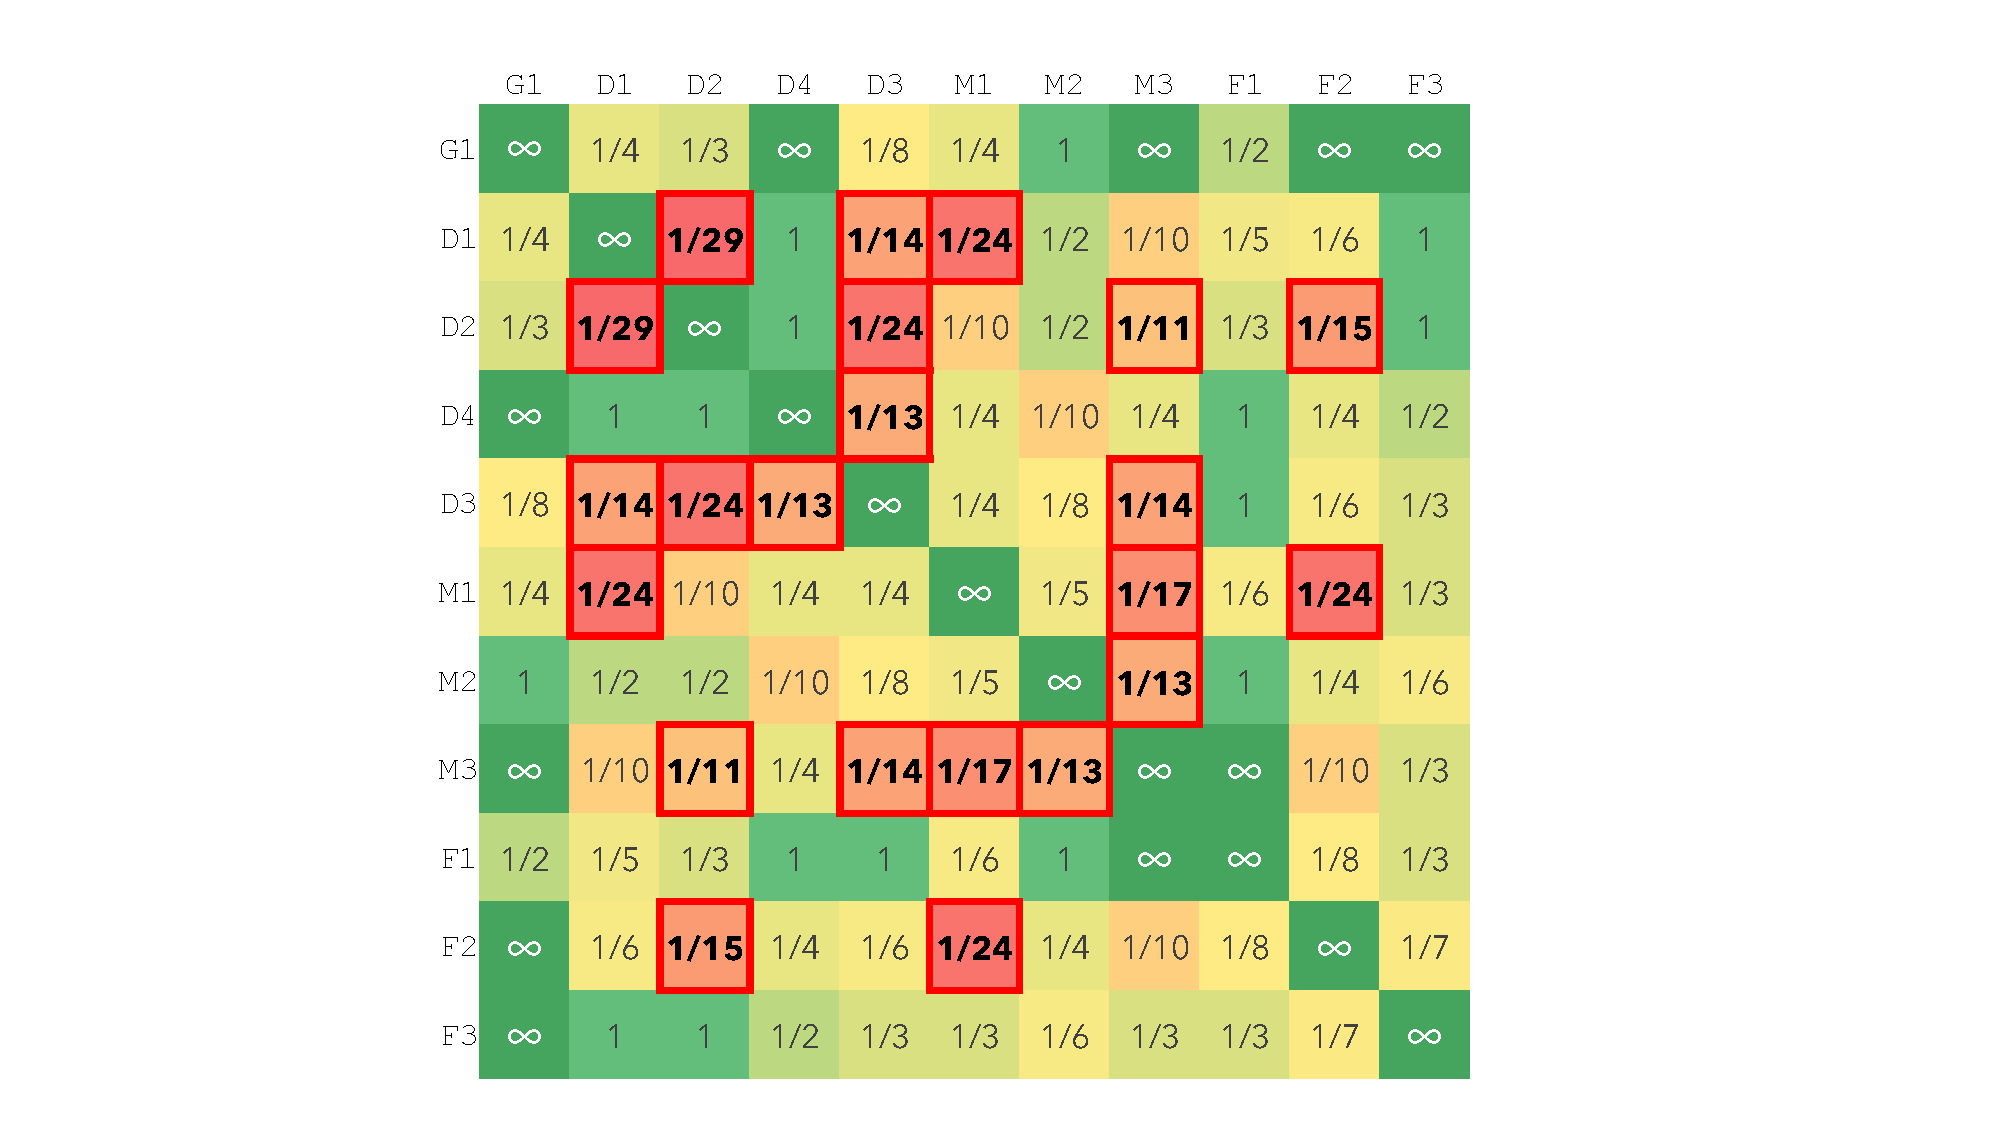
\includegraphics[width=.66\textwidth]{matrix_distance.pdf} 	% 图片相对位置
    \caption{Topological Distance Matrix of the 1\textsuperscript{st} match}		% 图片标题 
    \label{fig:matrix_distance}							% 图片标签
\end{figure}

First, we apply our model to the 1\textsuperscript{st} match and build the ball passing network. From the adjacency matrix, the \textit{Total Links} $L$ and \textit{Network Density} $\rho$ can be easily obtained by the equation \eqref{eq:total_links} and \eqref{eq:network_density} we give, which are 369 and 6.71 respectively. Moreover, we can use the equation \eqref{eq:topological_distance} to obtain the topological distance matrix (see \textbf{Figure \ref{fig:matrix_distance}}).


In the topological distance matrix, $\infty$ means the distance between the two nodes is infinite, which suggests that they don't have any passing in the game. There is no doubt that the statistics marked by red box is smaller than other statistic, which means the two nodes are very close in topological distance. 

In \textit{Graph Theory}, we call these nodes with \textit{higher similarity (distance) cluster}. Therefore, the passing network has many clusters in it and we use a \textit{K-means Algorithm}\upcite{5}  to classify the clusters in our passing network. The results have been shown in \textbf{Figure \ref{fig:K-means}}.

\begin{figure}[htbp]
    \centering
    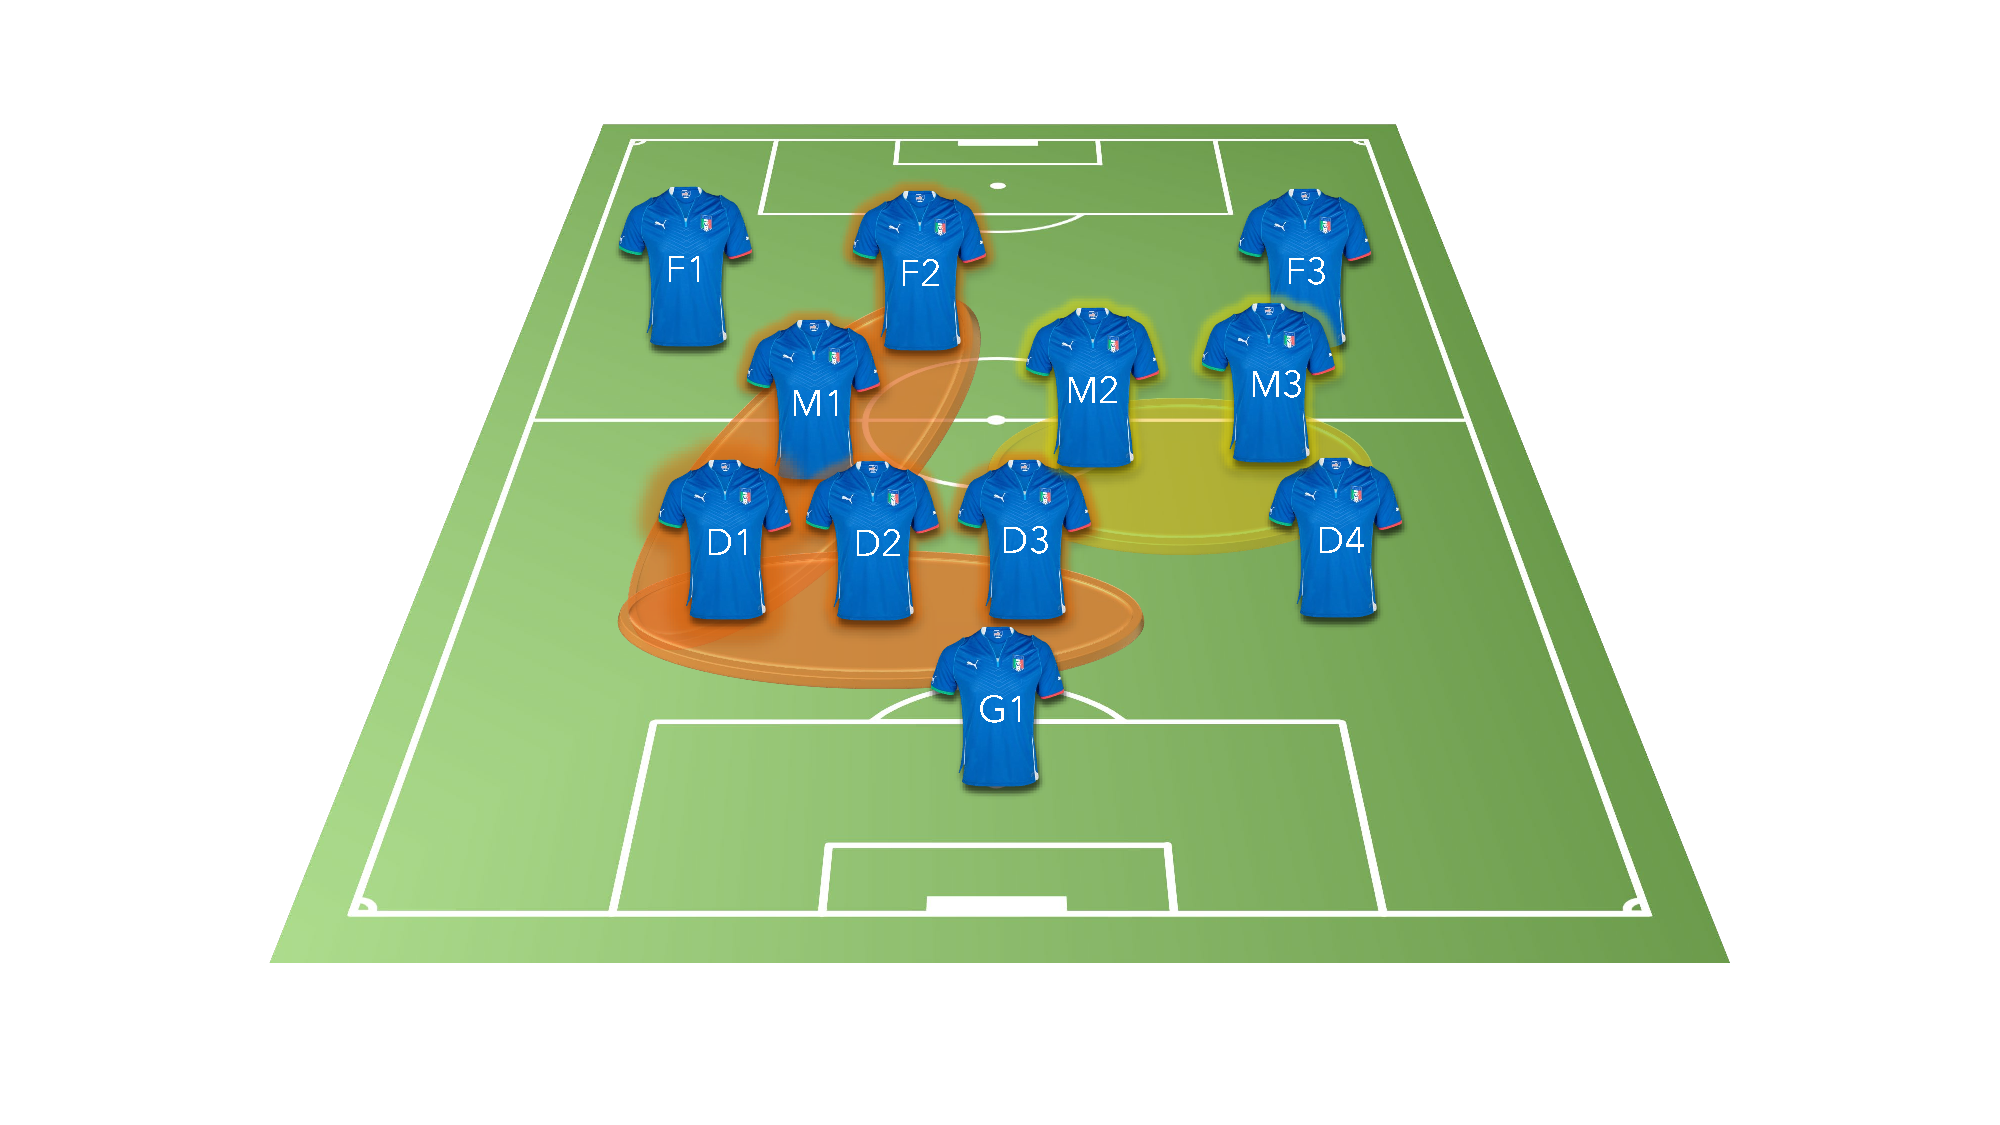
\includegraphics[width=.65\textwidth]{Dyadic_Triadic_Configurations.pdf} 	% 图片相对位置
    \caption{Dyadic and Triadic Configurations}		% 图片标题 
    \label{fig:K-means}							% 图片标签
\end{figure}

Consequently, we classify (\texttt{D1, D2, D3}), (\texttt{D1, M1, F2}) and (\texttt{M2, M3}) into three clusters, which are so-called \textit{Dyadic and Triadic Configurations}. Also, we can conclude that the passing network patterns involve one dyadic configuration and two triadic configurations. 

Then we explore more deeply on (\texttt{D1, M1, F2}). According to the passing network, these three players make 227 passes in total, while the passes between these three account for 26.7\%. Moreover, the \textit{cluster coefficient} $C$ of the three equals 7.31, much smaller than that of the whole team (7.62), which means the connectivity between the (\texttt{D1, M1, F2}) is much higher than that between the three and other players. In this case, it's more likely to form clusters just like these three players. 



\subsection{Other Structural Indicators}
\subsubsection{Time Scale}
In a gesture to explore other structured indicators to evaluate the ball passing network, we next analyse the time scale. As small as every minute and every second, and as large as the entire game and season, the \textit{time scale} can undoubtedly reflect the team's game status. In this part, we mainly discuss two aspects: \textit{10-minute network passes} and the \textit{entire game network passes}. 

\clearpage
\begin{itemize}
    \item \textbf{10-minute Network Passes}
\end{itemize}

When it comes to the relatively small period of time throughout the game, we have to introduce the \textit{tempo} in football. 
Tempo, in a word, is the speed of any movement or activity, which mainly includes the speed of advancement, transmission, and  running. Players in the field determine when to be fast and when to be slow through factors such as technology, vision, anticipation, tactics, and the actual situation of the game.

An important indicator of tempo is the number of passes. Team with more passes in a unit time are those generate more passes in less time, and indicates that they have a well capability of controlling tempo. In our case, we analyzed the effects of using different time intervals $t$ of passes and chose $t = 10 \,\mathrm{min}=600\,\mathrm{sec}$ as a trade-off value. 

At the same time, we take the 1\textsuperscript{st} match as an example to study the number of passes of the Huskies every ten minutes, which is defined as $\alpha$. Considering the interval between two half, we didn't talk about the number of ball passes between 40 - 45 min in both half. 

\begin{figure}[htbp]
    \centering
    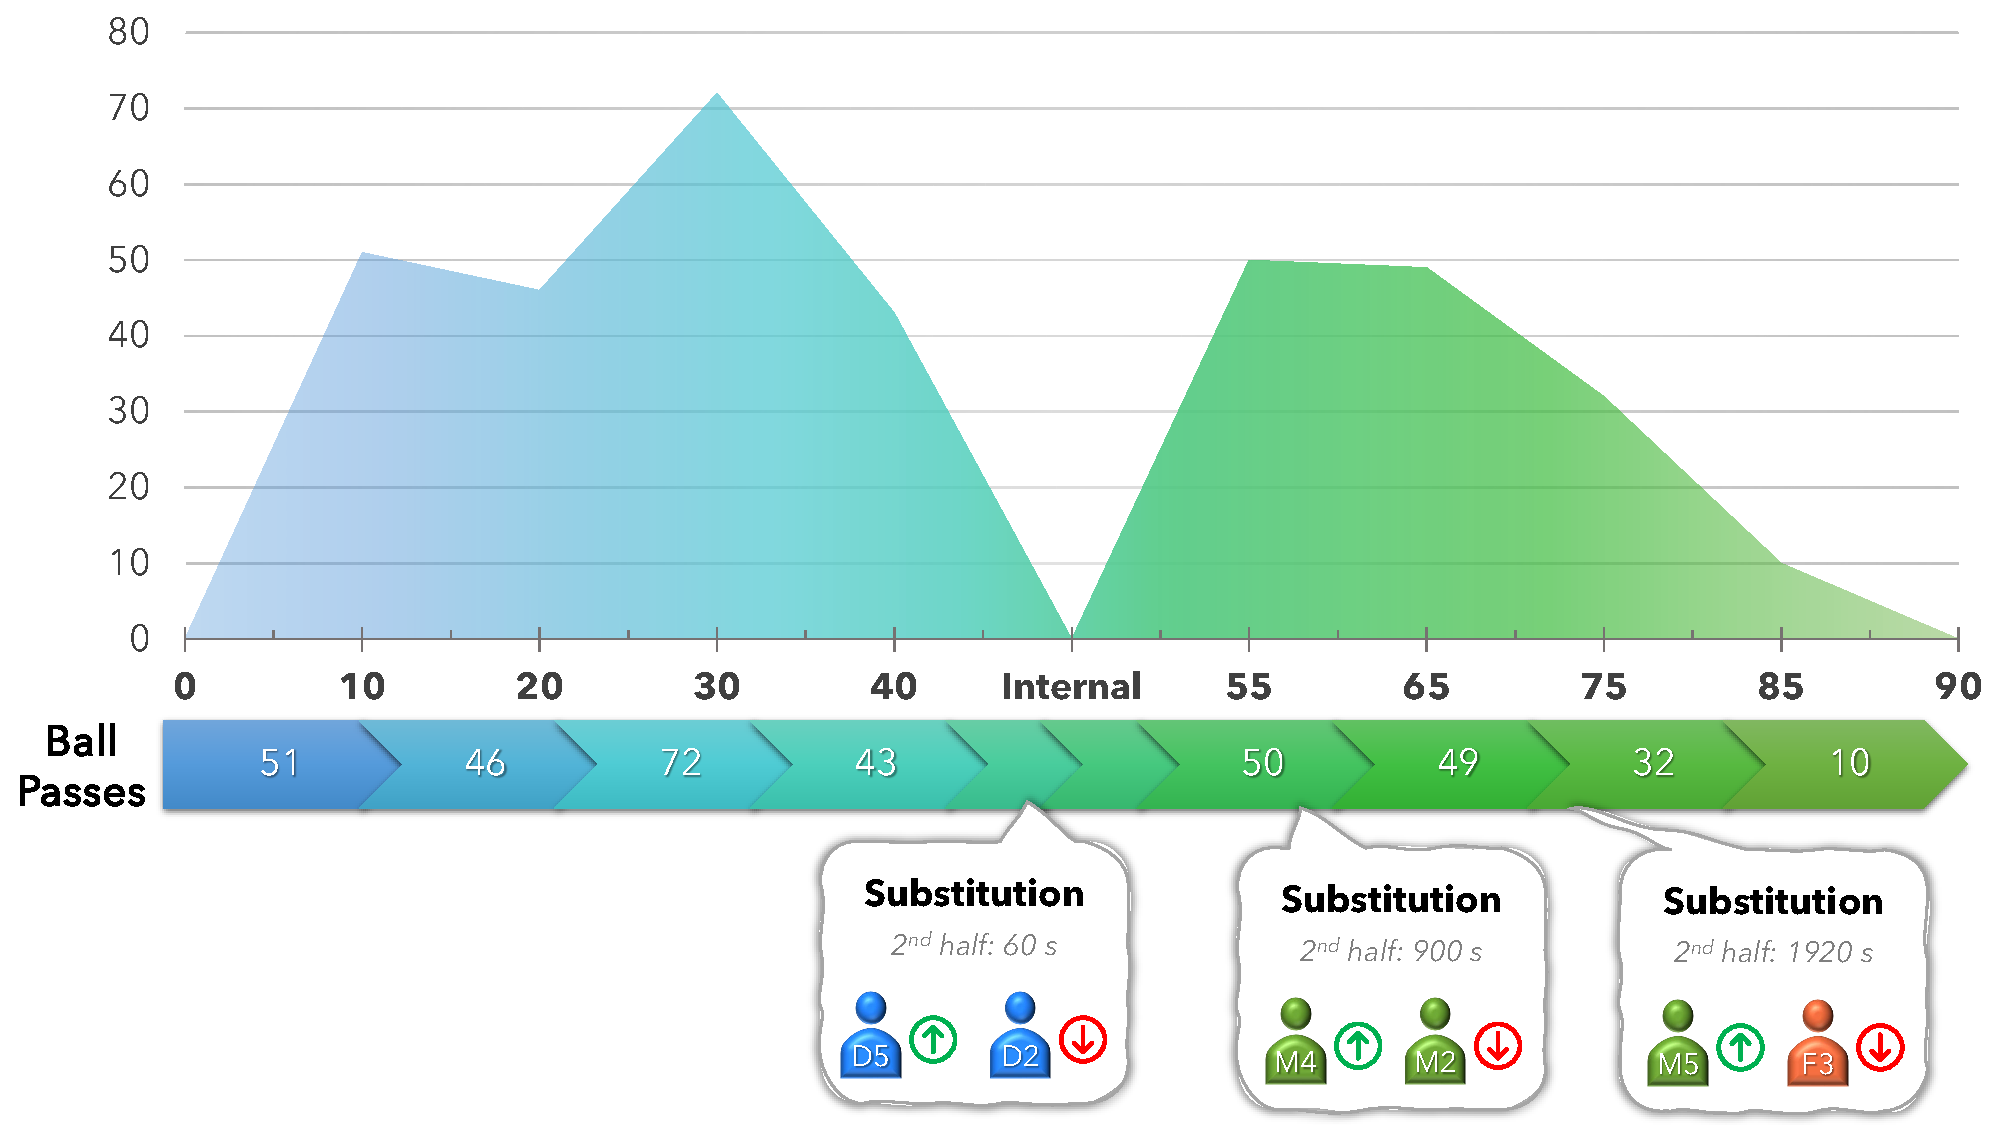
\includegraphics[width=.9\textwidth]{timeline_match1.pdf} 	% 图片相对位置
    \caption{10-minute Network passes of Huskies in the 1\textsuperscript{st} match}		% 图片标题 
    \label{fig:timeline_match1}							% 图片标签
\end{figure}

As is clearly depicted in \textbf{Figure \ref{fig:timeline_match1}}, Huskies' 10-minute Network passes is relatively stable. From the timeline, we can find that in about 30 minutes, the Huskies changed the tempo, the attack speed accelerated, and the rhythm showed a simple and bright. In the last 10 minutes, the Huskies were relatively conservative and had fewer passes, and we can attribute it to exhaust.


\vspace{4pt}
\begin{itemize}
    \item \textbf{Entire Game and Entire Season Network Passes}
\end{itemize}

In this part, we explore the passing network at the level of the whole game. Using the ball passing matrix and equation \eqref{eq:total_links}, we get the following \textbf{Figure \ref{Fig:total_links}}.



Six matches are chosen from different period of the whole season. As is shown in \textbf{Figure \ref{Fig:total_links}}, we can conclude that at the beginning of the season, the teamwork performance is \textit{unstable}. 


\begin{figure}[htbp]
    \centering    
    \subfigure[Match 1 ($L=369$)]{				% 图片1([]内为子图标题)
    \label{Fig.sub.match1}							% 子图1的标签
    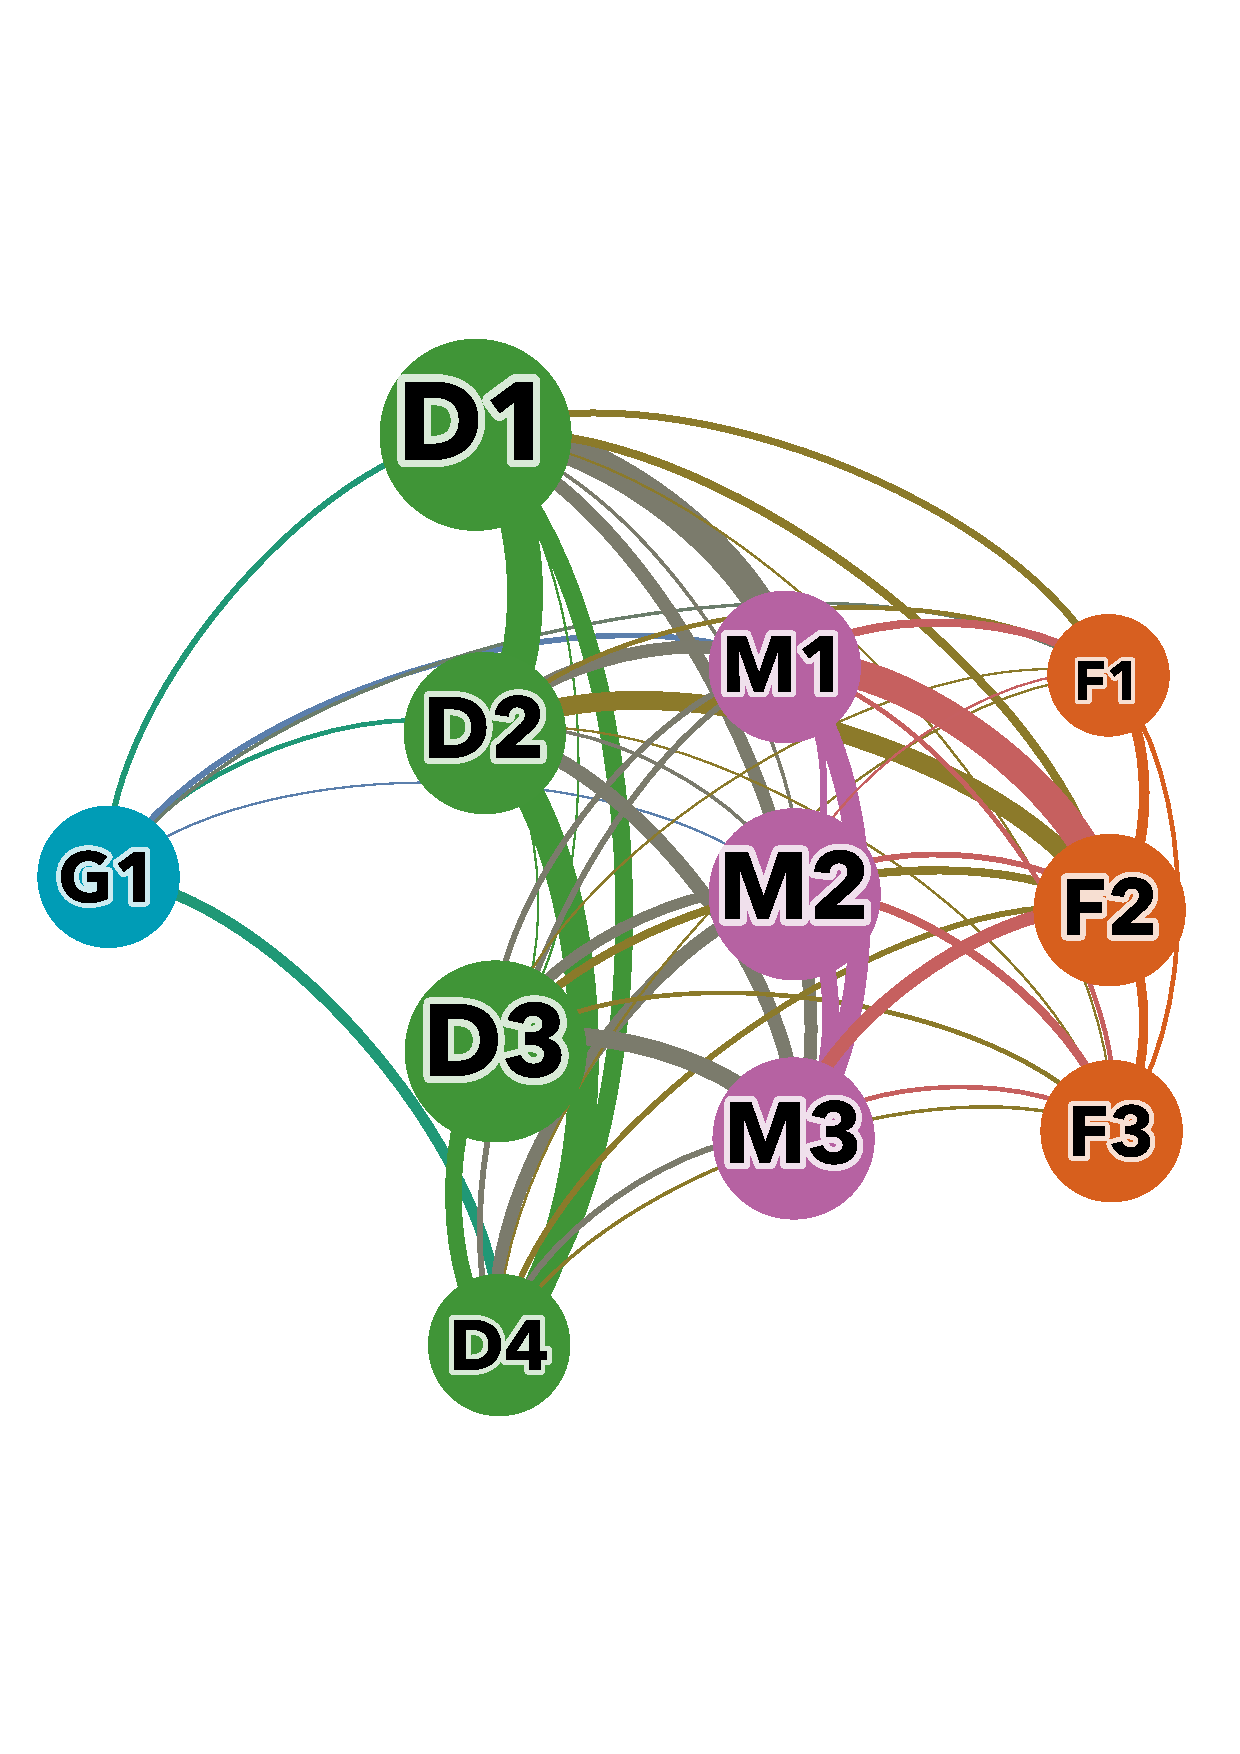
\includegraphics[width=0.32\textwidth]{match1_network.pdf}}			  % 子图1的相对位置
    \subfigure[Match 2 ($L=180$)]{				% 图片2
    \label{Fig.sub.match2}						% 子图2的标签
    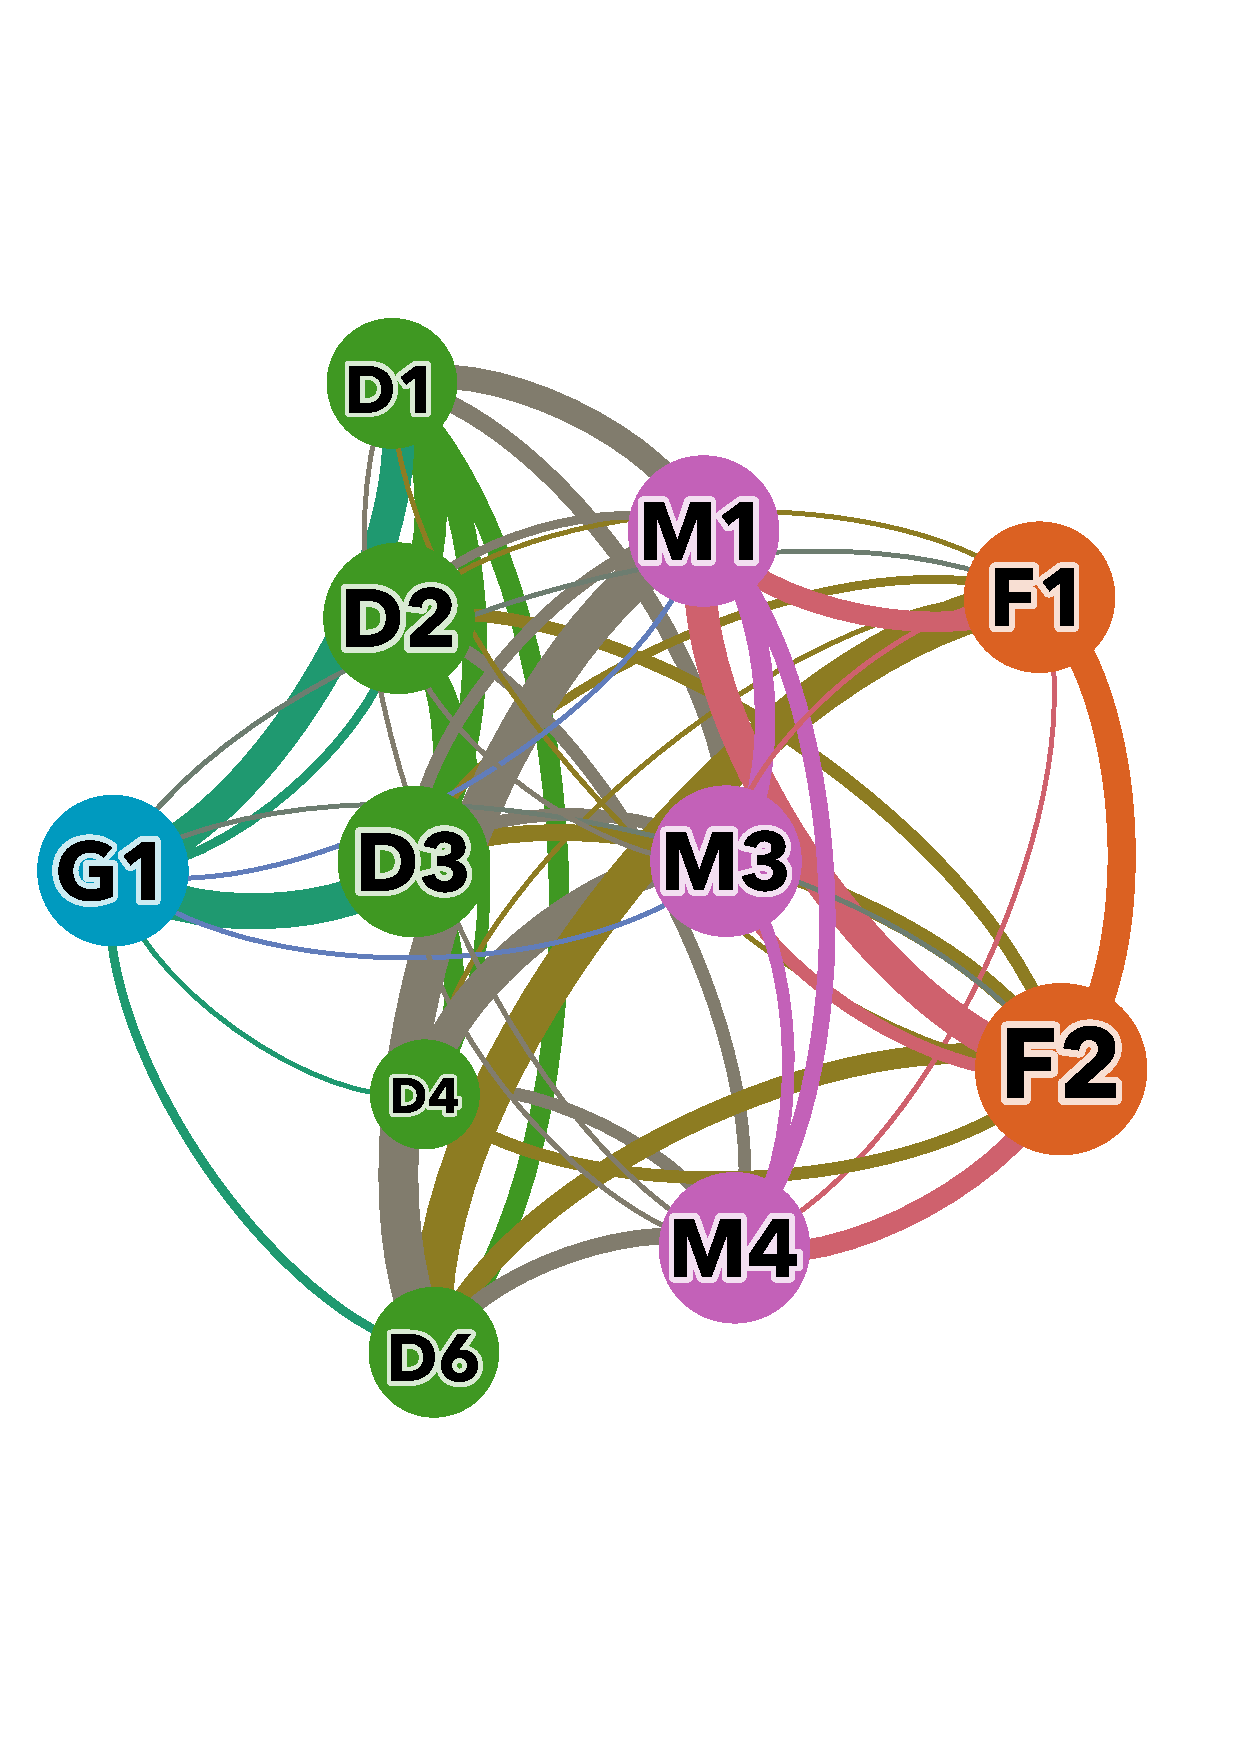
\includegraphics[width=0.32\textwidth]{match2_network.pdf}}
    \subfigure[Match 3 ($L=324$)]{				% 图片1([]内为子图标题)
    \label{Fig.sub.match3}							% 子图1的标签
    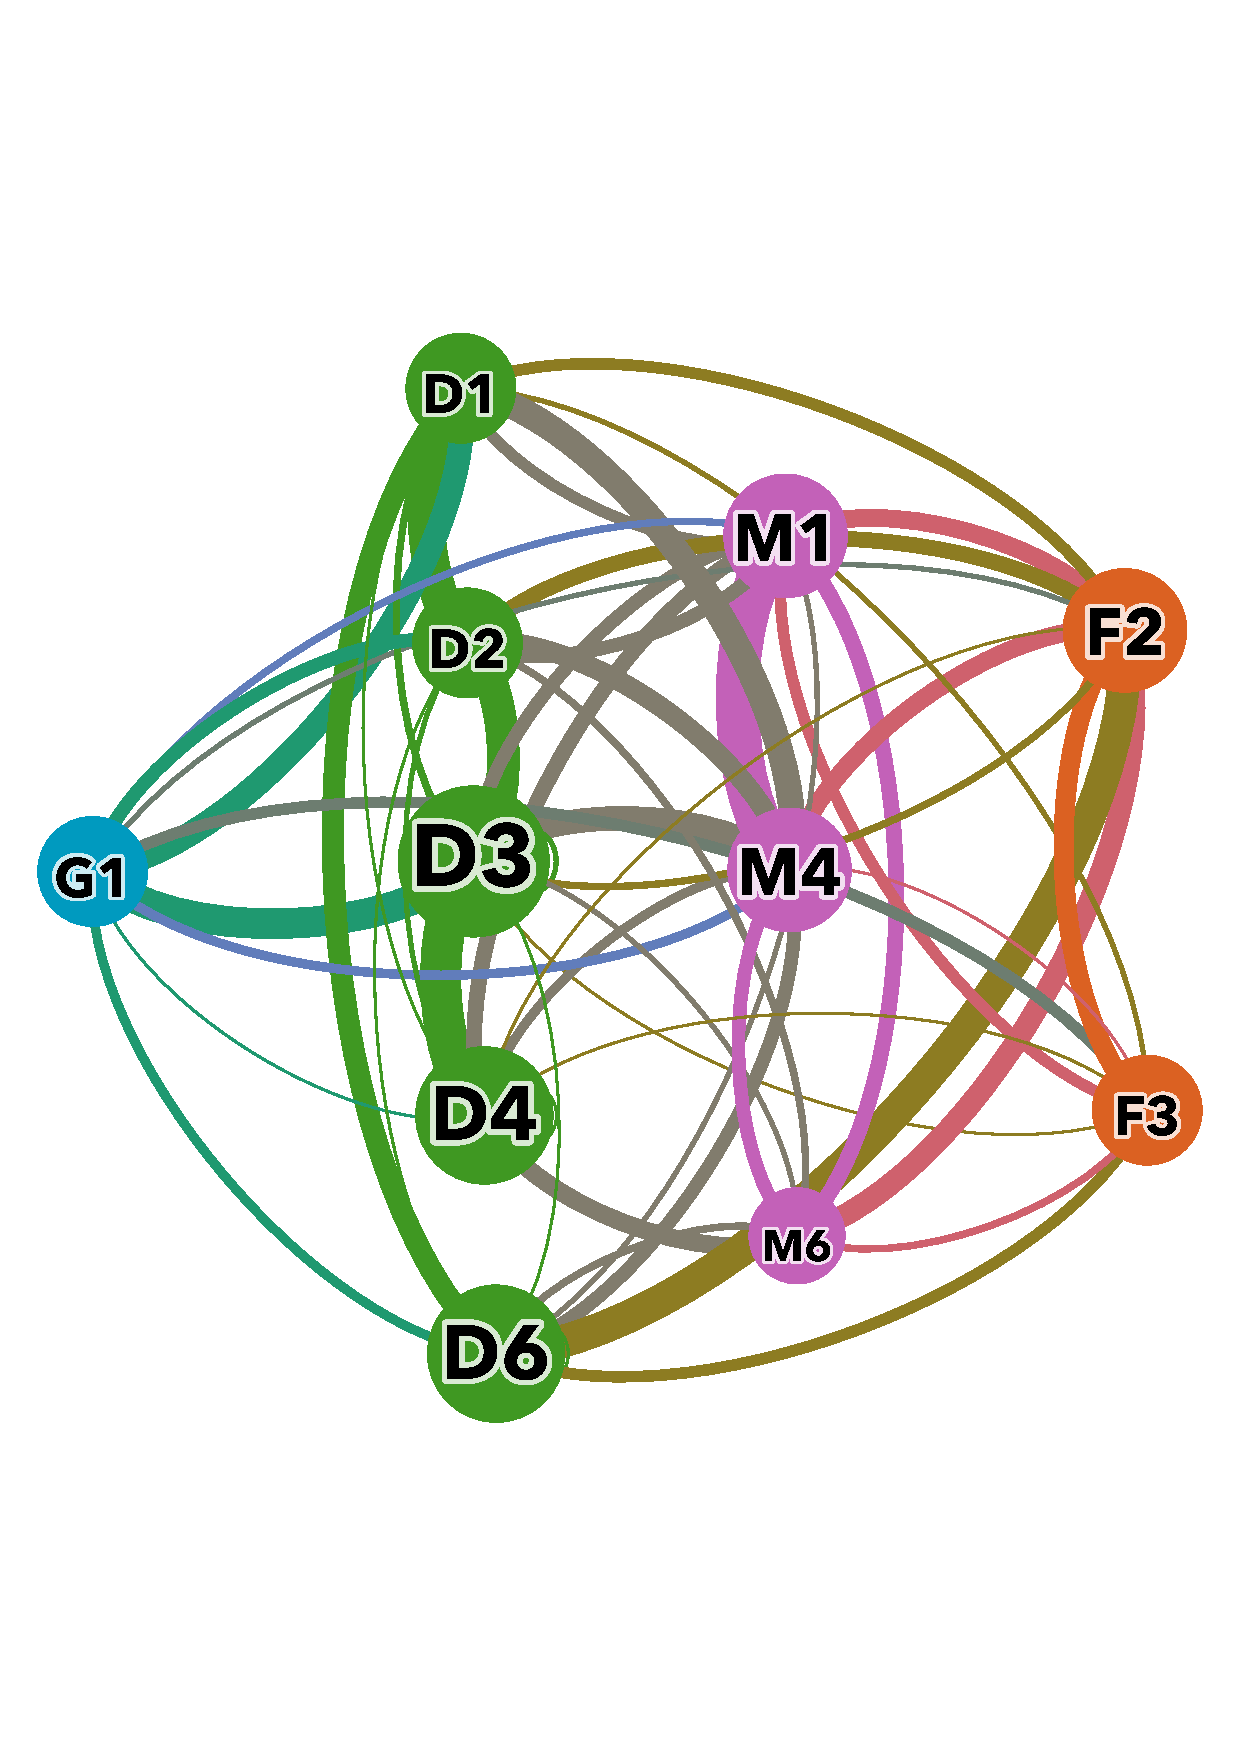
\includegraphics[width=0.32\textwidth]{match3_network.pdf}}			  % 子图1的相对位置
    
    \subfigure[Match 4 ($L=354$)]{				% 图片2
    \label{Fig.sub.match4}						% 子图2的标签
    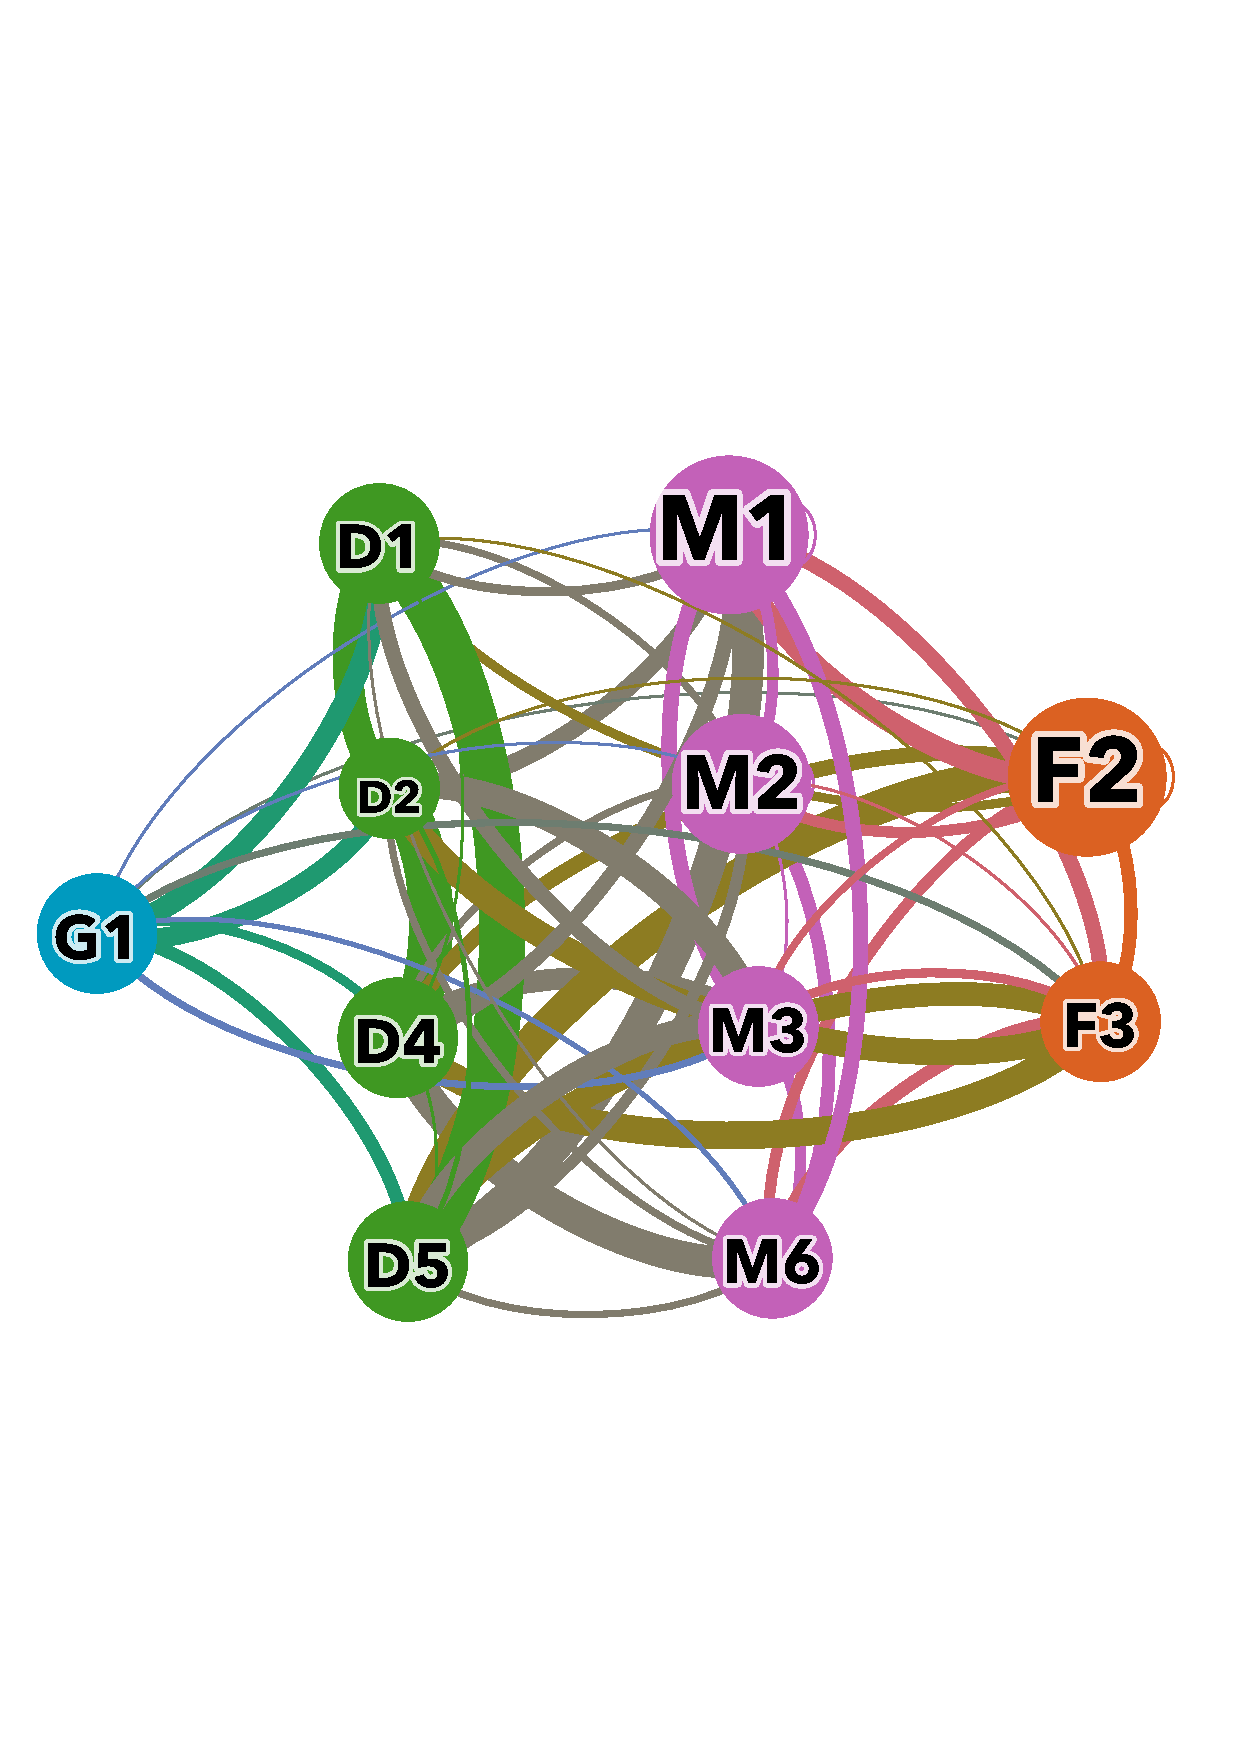
\includegraphics[width=0.32\textwidth]{match4_network.pdf}}
    \subfigure[Match 10 ($L=359$)]{				% 图片1([]内为子图标题)
    \label{Fig.sub.match10}							% 子图1的标签
    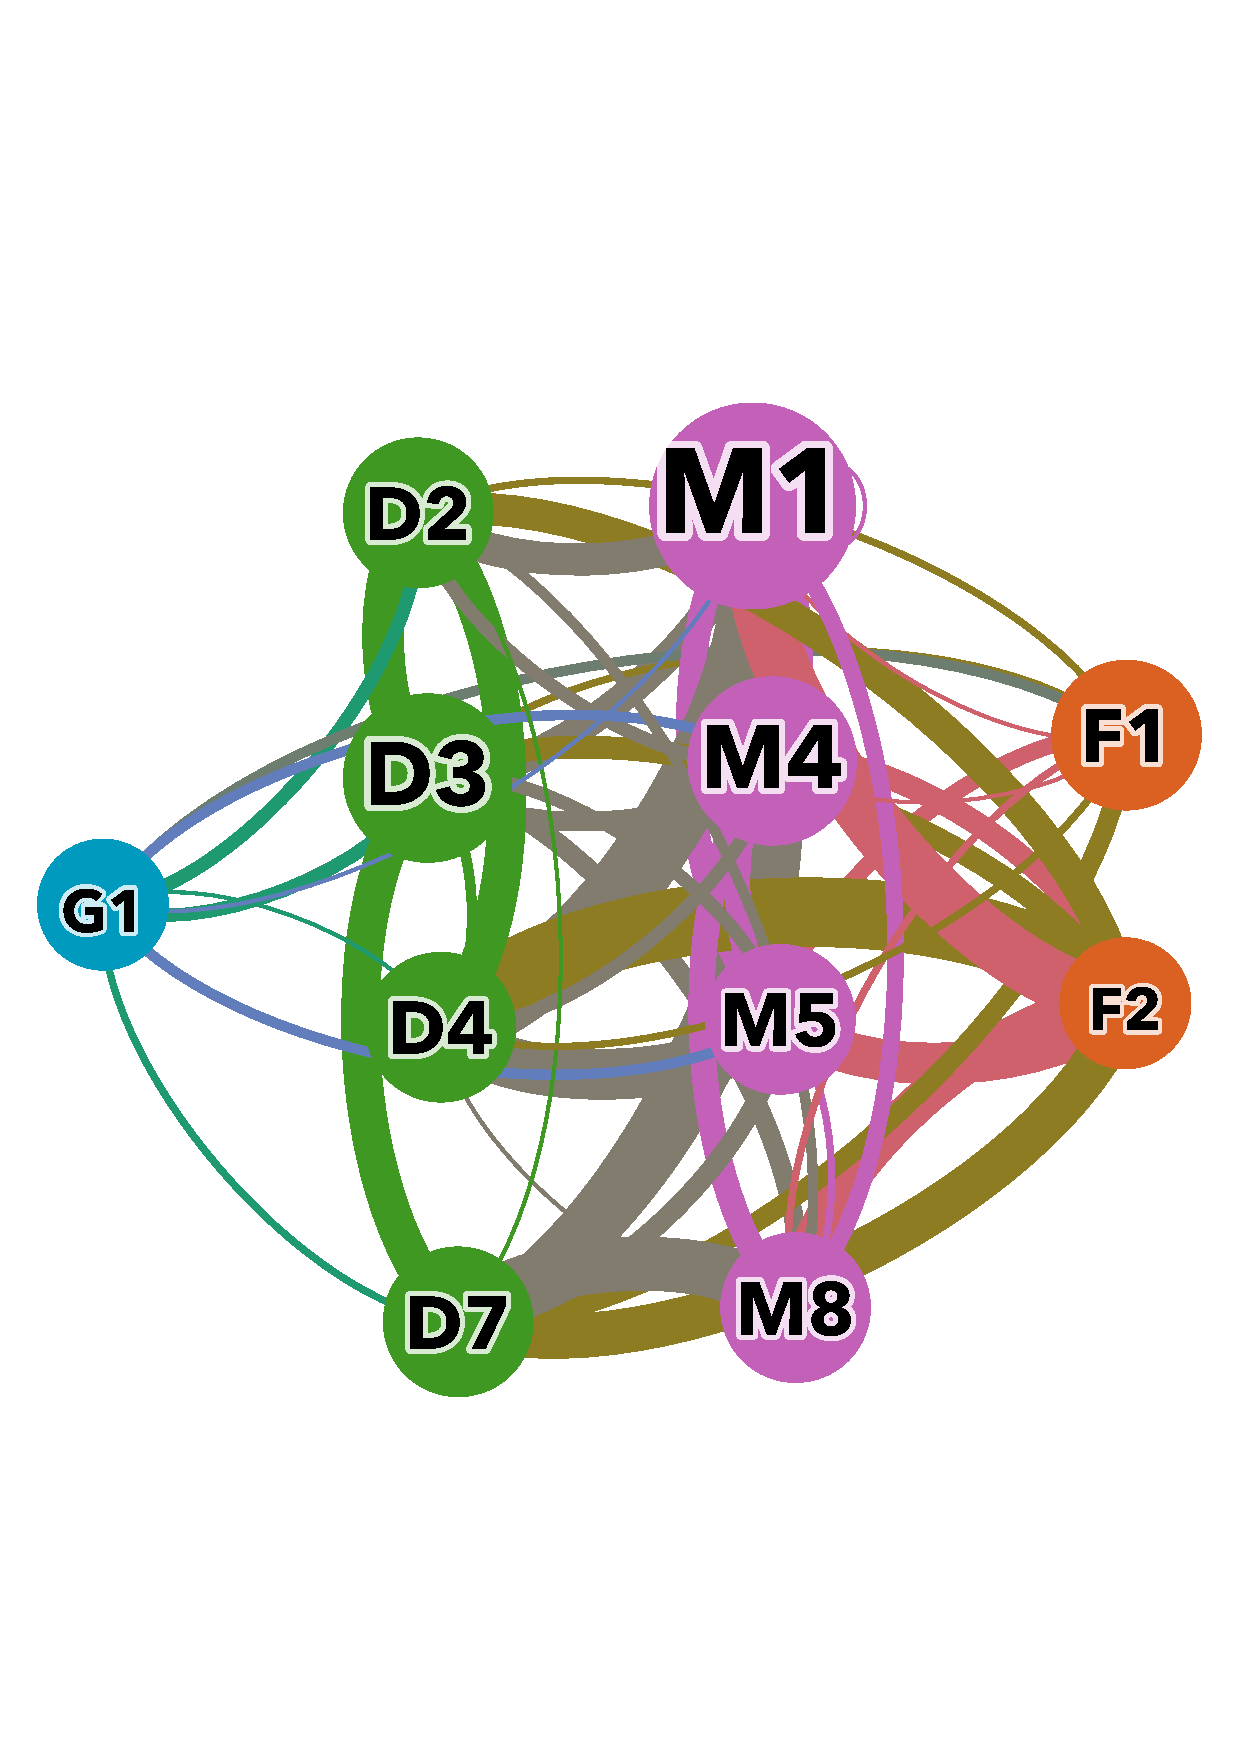
\includegraphics[width=0.32\textwidth]{match10_network.pdf}}			  % 子图1的相对位置
    \subfigure[Match 13 ($L=347$)]{				% 图片2
    \label{Fig.sub.match13}						% 子图2的标签
    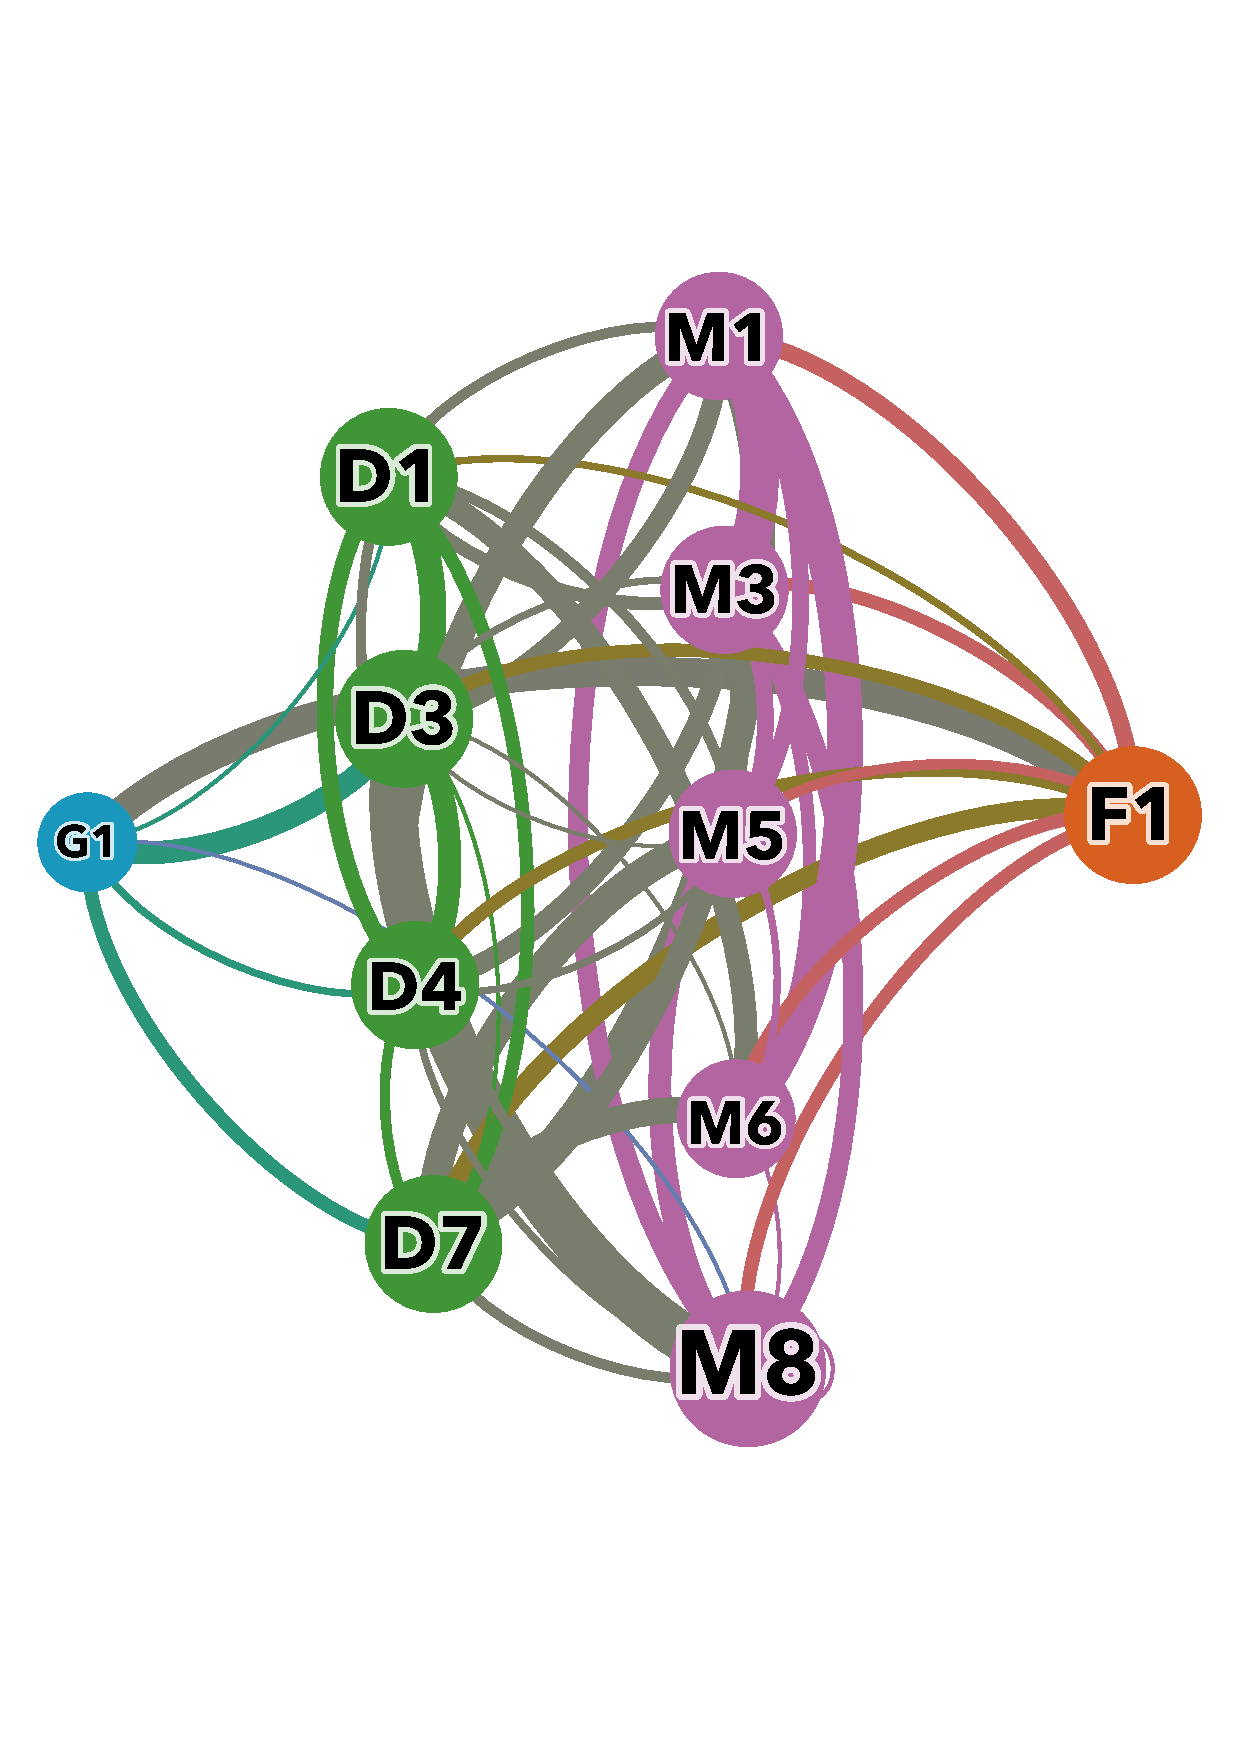
\includegraphics[width=0.32\textwidth]{match13_network.pdf}}
    \caption{Entire Game and Entire Season Network Passes}		% 总图标题
    \label{Fig:total_links}									% 总图标签
\end{figure}


However, As the season progresses, the Huskies' performance has gradually stabilized, and a stronger connectivity between the players has also formed. 


\subsubsection{Region Scale}
In spite of time scale, we can also analyze the passing network by region scale. The football field can be divided into eight regions averagely. Then we use the location where each passes occur to have an overview.
\begin{figure}[htbp]
    \centering
    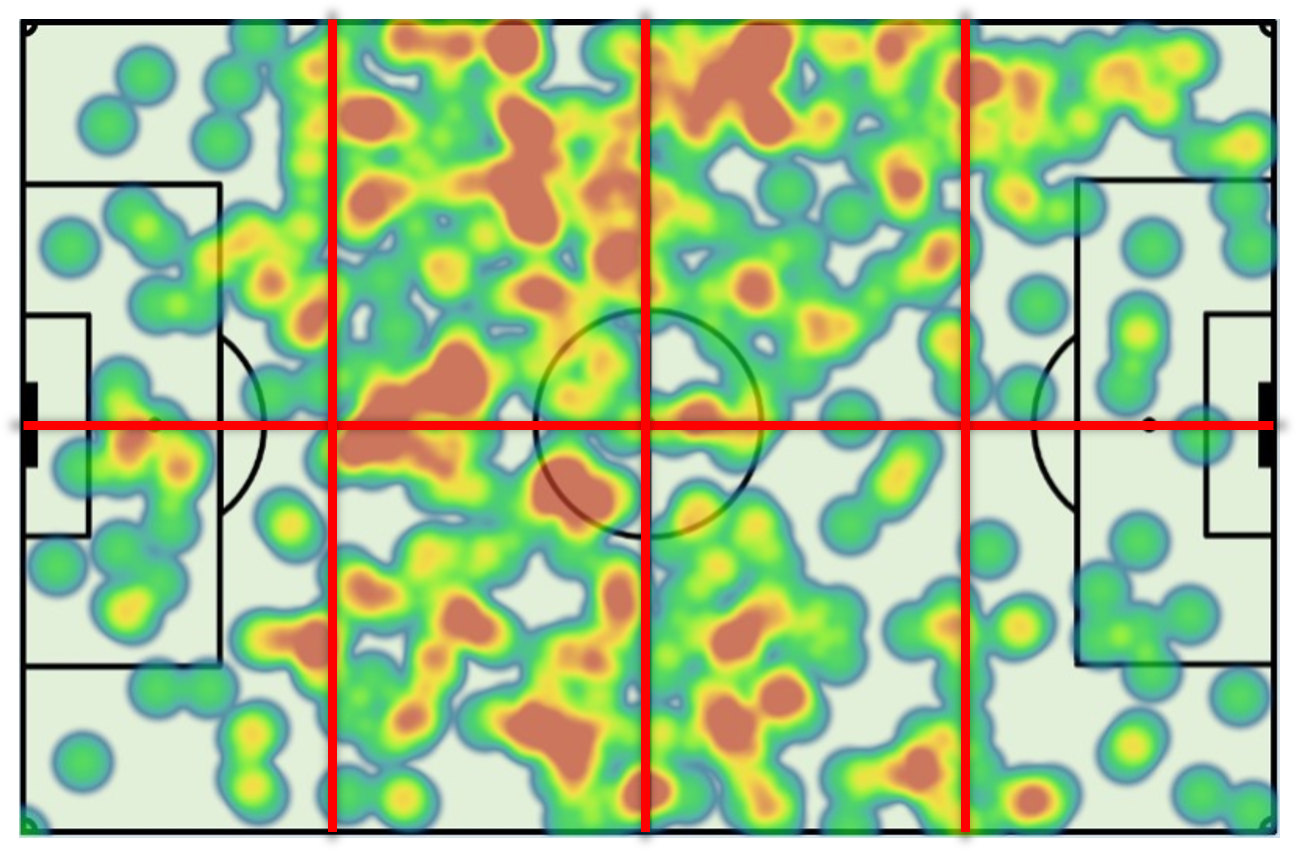
\includegraphics[width=.5\textwidth]{task1_hotmap.png} 	% 图片相对位置
    \caption{An overview of the passes in football field}		% 图片标题 
    \label{fig:task1_hotmap}							% 图片标签
\end{figure}

As is shown in \textbf{Figure \ref{fig:task1_hotmap}}, Huskies make their most passes in the backcourt, which is in line with their highlight in defense. Moreover, the connectivity between defense players is higher than that of forward players. However, \textbf{Figure \ref{fig:task1_hotmap}} also shows that Huskies hasn't made full use of the width of the field. They can try to make more passes in those regions with light color. 



\section{\textsc{Task 2: } Evaluation of Successful Teamwork}
\subsection{Identification of Performance Indicators}
To further evaluate whether the teamwork is success, we should select some relevant indicators. This paper simplifies the performance indicators into two aspects: \textit{Static} and \textit{Dynamic}. The \textit{Static} performance indicators mainly contain: \textit{Coordination among players}, \textit{Distribution of contributions}. And the \textit{Dynamic} performance indicators involve: \textit{tempo}, \textit{flexibility}, \textit{Pressing}.

\subsubsection{Static Layer}
\begin{itemize}
    \item \textbf{Coordination among players}
\end{itemize}

In terms of coordination among players, we use \textit{cluster coefficient} $C$ to quantify it. One player's cluster coefficient means his connectivity with other teammates. The team's average cluster coefficient embodies the level of coordination in the team. Therefore, the higher average cluster coefficient $C$ is, the stronger coordination $\gamma$ is. 

\vspace{4pt}
\begin{itemize}
    \item \textbf{Distribution of contributions}
\end{itemize}

Considering the contribution distribution, we may consider the contribution of each player into two aspects, namely forward and defense. Set the number of shots per player $i$ to $\mu_i$ and the number of defenses to $\nu_1$.
% \begin{table}[!htbp]
%     \begin{center}
%     \caption{Distribution of contributions}
%     \begin{tabular}{c|cccccccccccc}
%         \toprule
%         Player  & 1 & 2 & 3 & 4 & 5 & 6& 7 & 8 & 9 & 10 & 11 &Sum\\
%         \midrule
%         \textbf{Forward} & $\mu_1$ & $\mu_2$& $\mu_3$& $\mu_1$ & $\mu_2$& $\mu_3$& $\mu_1$ & $\mu_2$& $\mu_3$&$\mu_{10}$&$\mu_{11}$&$\mu_{sum}$ \\
%         \textbf{Defense} & 1000& $\mu_1$ & $\mu_2$& $\mu_3$& $\mu_1$ & $\mu_2$& $\mu_3$& 1800&5000&8000&15000&20000 \\
%         \bottomrule
%     \end{tabular}\label{tb:match1_distribution}
%     \end{center}
% \end{table}

Below we discuss forward and defense success rates. Forward success rate can be obtained by the ratio of the number of goals to the number of shots, which can be described as:
\begin{equation}
    f=\frac{\mu_{\mathrm{goal}}}{\sum_{i=1}^{11}\mu_i},
\end{equation}

Defense success rate can be obtained by the ratio of the number of defenses to the number of losses plus one, which can be expressed as:
\begin{equation}
    d=\frac{\sum_{j=1}^{11}\nu_j}{\nu_{\mathrm{loss}}+1}.
\end{equation}
Where we add one to the denominator of $f$ to prevent the denominator from being zero.

Then we get a parameter $\varphi$ about \textit{Distribution of contributions}:
\begin{equation}
    \varphi=f\cdot d.
\end{equation}
Where Larger $\varphi$ means fewer mistakes and more success.

\subsubsection{Dynamic Layer}
\begin{itemize}
    \item \textbf{Tempo}
\end{itemize}

In \textbf{\textsc{Task 1}}, we have talked about tempo by means of \textit{10-minute Network Passes}, which is the number of passes per ten minutes. However, when we discuss team performance evaluation, the performance of \textit{10-minute Network Passes} is not very obvious, we choose \textit{50-ball Passing Time}\upcite{6}. We construct the \textit{50-ball Passing Time} with the aim of accounting for the temporal evolution of the game. \textit{50-ball Passing} contain only 50 consecutive passes and are assigned the time of the last of these passes.

The 50-ball Passing Time $t_{b}$ is the time required to construct a 50 ball passes. It is obtained subtracting the time of the first pass of the network from the time of the last pass. Teams with shorter $t_b$ are those that generate more passes in less time.

\vspace{4pt}
\begin{itemize}
    \item \textbf{Flexibility}
\end{itemize}

In this section, we use the $y$-coordinate standard deviation $\sigma_y$ to represent team \textit{flexibility}. The better the team's flexibility, the greater the standard deviation $\sigma_y$, and the more the off-center disturbances occur. The flexibility can be marked as:
\begin{equation}
    \sigma_y=\frac{1}{n}\sum_{j=1}^{n}(y_j-\bar{y})
\end{equation}

As is shown in \textbf{Figure \ref{Fig:Flexibility}}, the team with higher $\sigma_y$ has more attack strategy, either from both sides or in the middle. In contrast, the team with smaller $\sigma_y$ has fewer attack strategy. As a result, if the opponents focus on the defense of the middle, they will not be flexible enough to change their attack strategy like attacking from left or right. 
\begin{figure}[htbp]
    \centering    
    \subfigure[Match with higher Flexibility $\sigma_y=33.70$]{				% 图片1([]内为子图标题)
    \label{Fig.sub.Flexibility_33.70}							% 子图1的标签
    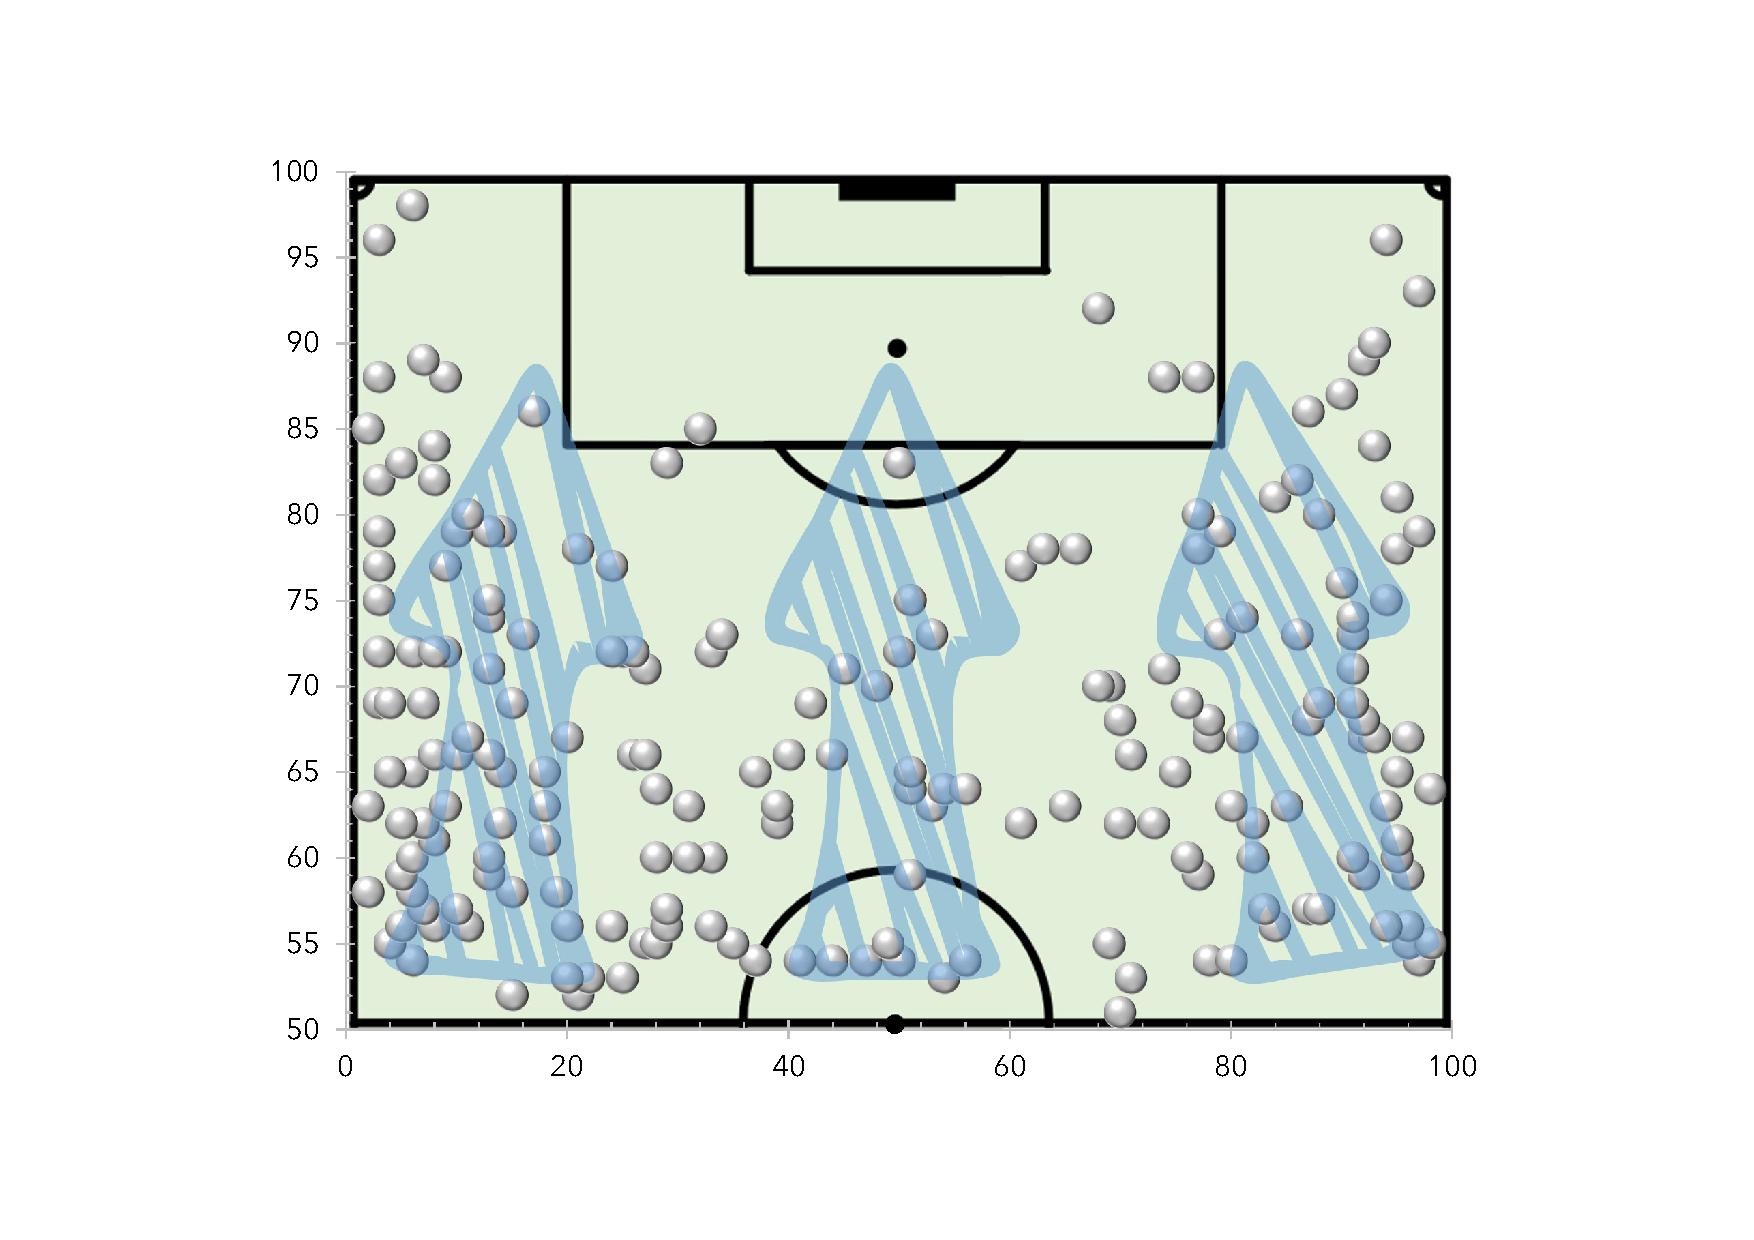
\includegraphics[width=0.45\textwidth]{Flexibility_3370.pdf}}			  % 子图1的相对位置
    \subfigure[Match with smaller Flexibility $\sigma_y=26.66$]{				% 图片2
    \label{Fig.sub.Flexibility_26.66}						% 子图2的标签
    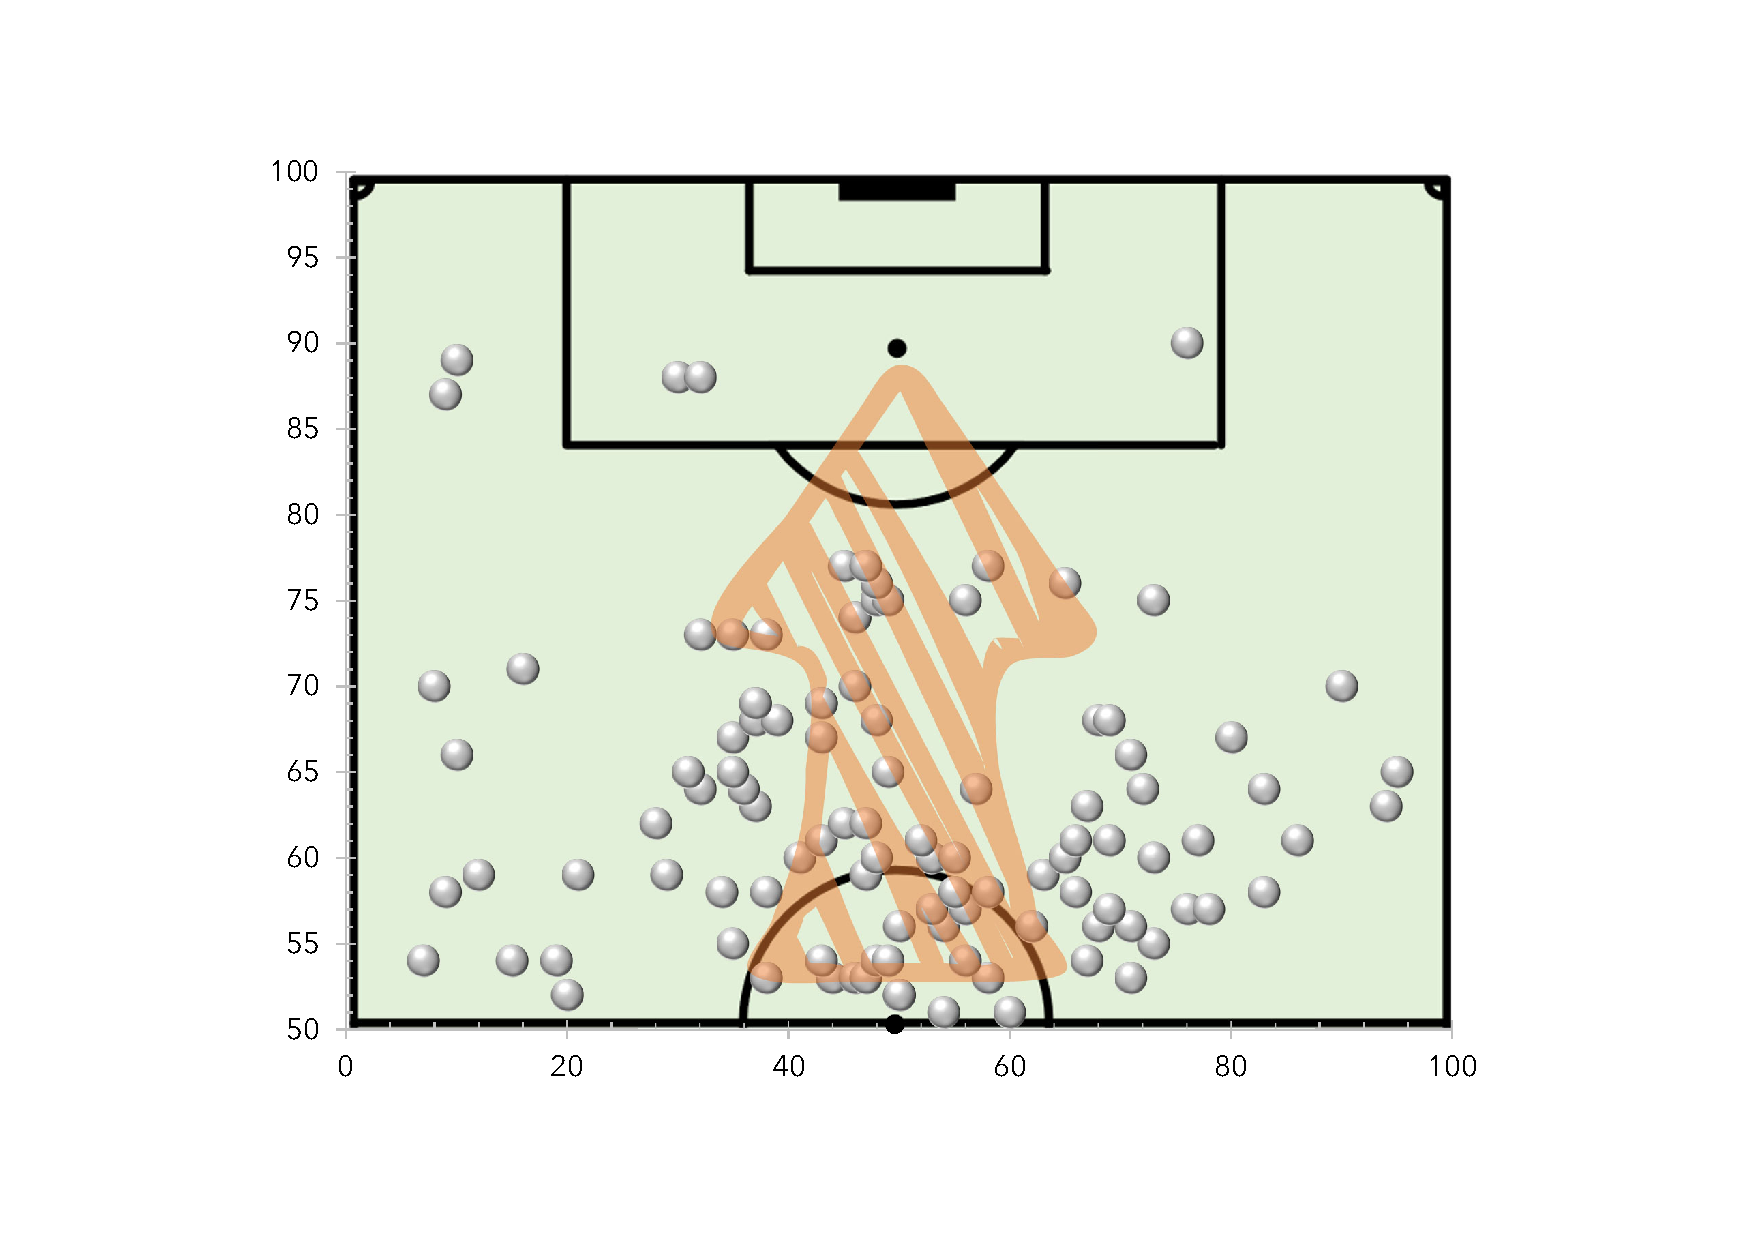
\includegraphics[width=0.45\textwidth]{Flexibility_2666.pdf}}
    \caption{Comparison of matches with different flexibility}		% 总图标题
    \label{Fig:Flexibility}									% 总图标签
\end{figure}



\begin{itemize}
    \item \textbf{Pressing}
\end{itemize}

\textit{Pressing} is an indicator of offense and defense status. \textit{Gegenpressing} refers to the premise of the entire defense of the team, forcing the opponent to rush the ball from the opponent's backcourt. Pressing can be estimated by the expectation of the $x$-coordinate. 
\begin{equation}
    \bar{x}=\frac{1}{n}\sum_{i=1}^{n}x_i
\end{equation}

When $\bar{x} = 50$, we can consider that there is no gegenpressing and the situation on the court is balanced; when $\bar{x}> 50$, there is a situation of gegenpressing on football field.

\begin{figure}[htbp]
    \centering
    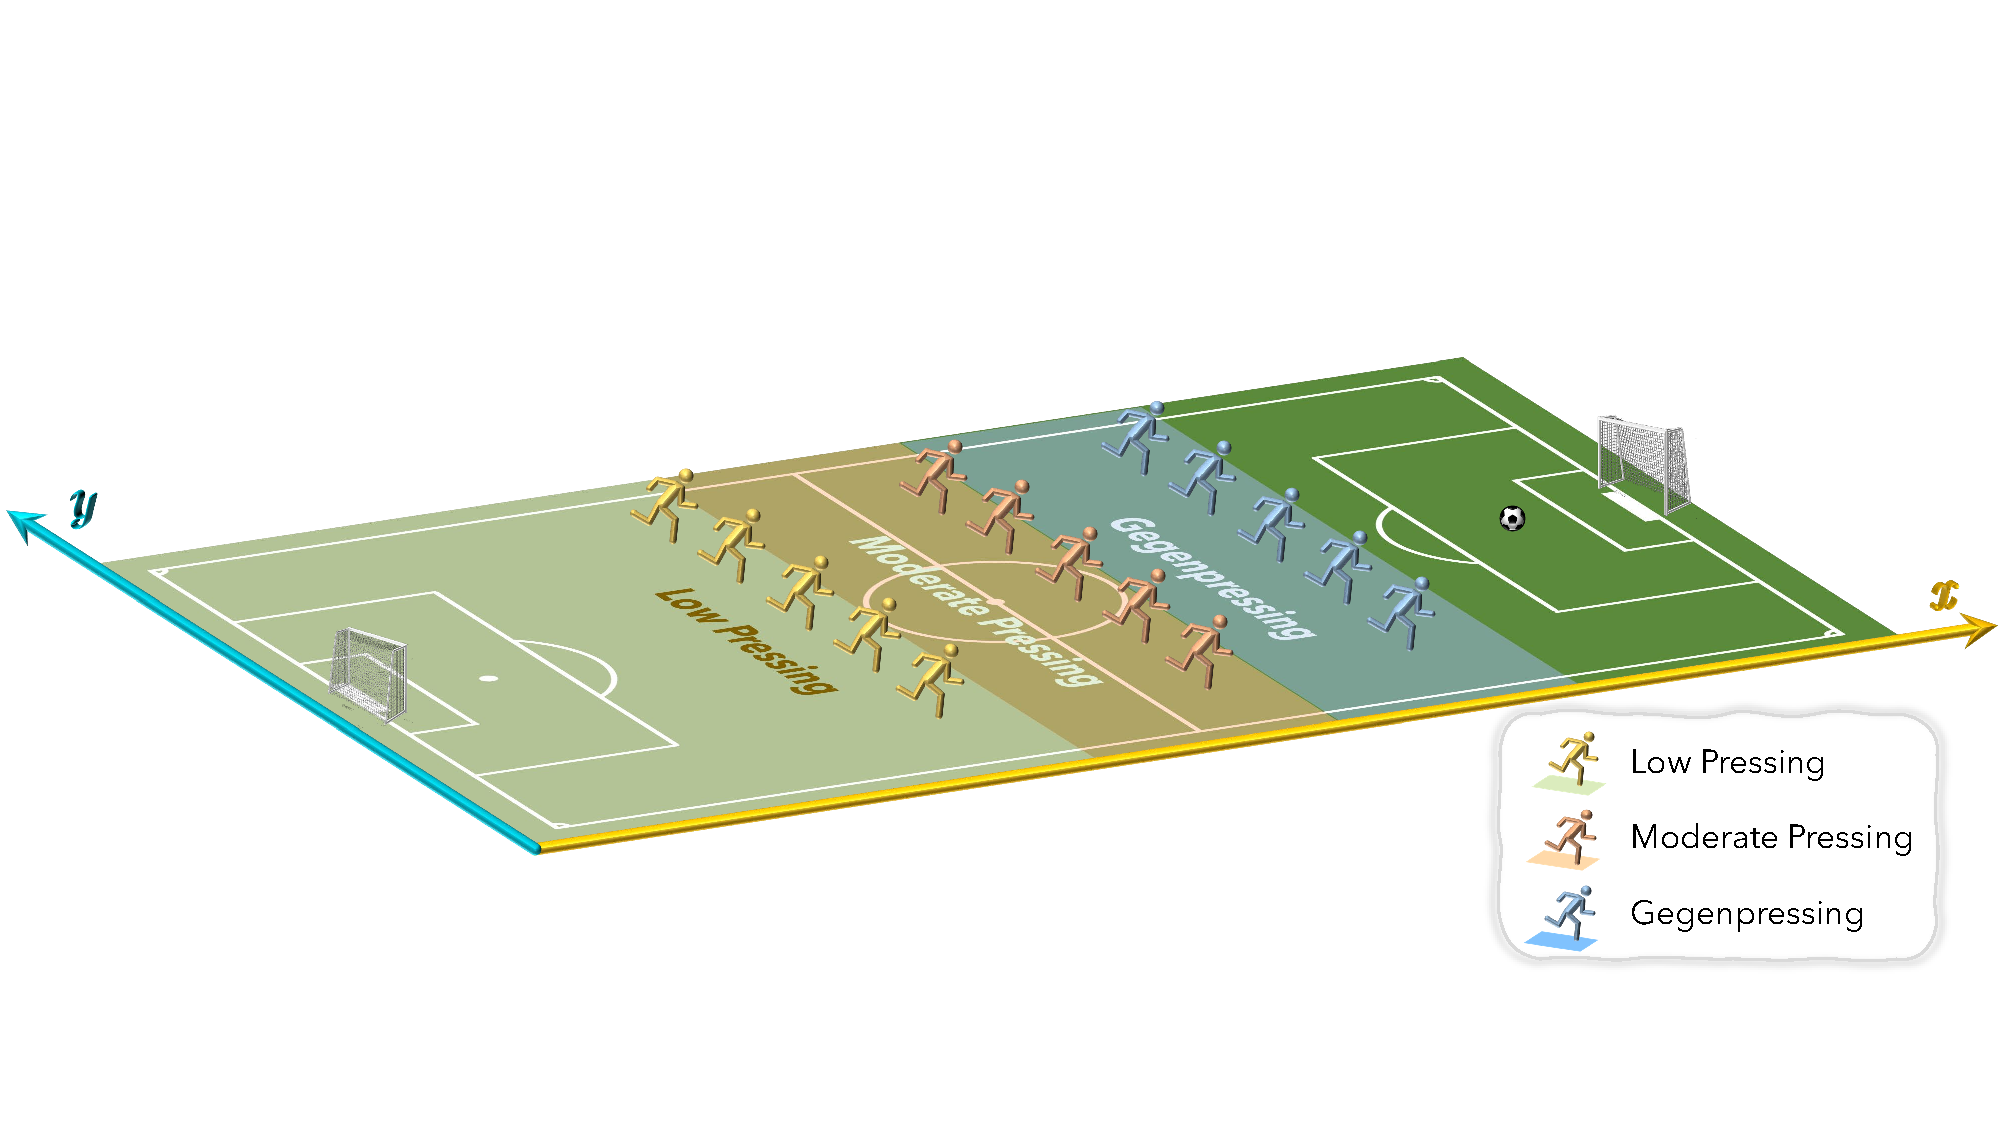
\includegraphics[width=1.0\textwidth]{Gegenpressing.pdf} 	% 图片相对位置
    \caption{Situation of Gegenpressing on football field}		% 图片标题 
    \label{fig:Gegenpressing}							% 图片标签
\end{figure}


\subsection{Evaluation model based on Adversarial Regression}
We describe the performance of a team $S$ during a football game by five network measures extracted from its passing network:  $x_1$ (\textit{Coordination among players} $\gamma$),
$x_2$  (\textit{Distribution of contributions} $\varphi$),
$x_3$  (\textit{Tempo} $t_b$),
$x_4$  (\textit{Flexibility} $\sigma_y$),
$x_5$  (\textit{Pressing} $\bar{x}$). We compute the \textit{five} network measures of teams for every game and observe a correlation among the proposed network measures and the success of a team during the competition, and therefore set up a simulation experiment to validate our approach. 
% In order to capture different aspects of Huskies's teamwork, here we establish \textit{Evaluation Model based on Adversarial Regression}. In order to consider whether the tactics applied by the team are universally effective or dependent on opponent's counter-strategies, so in each game, we also serve as the opponent. To build a model of performance and evaluate it, use this confrontational idea to establish a regression model, calculate the weight of each indicator, and serve as an evaluation model that can eventually capture the team's lineup, configuration, and dynamic positioning.

% We compute the five performance indicators for each matches provided and observe a correlation among the proposed performance indicators and the success of the Huskies during the competition. Thus, simulation experiments were established to verify our method. In the simulation, the outcome of each matches is predicted based on the value of the performance indicators of the two teams.
 We simulate the result of the match $i$ of the Huskies (or the opponent) through the following five steps:
\begin{enumerate}[\bfseries \textit{Step} 1:]
    \item For each of the two teams, we compute the score $S$ of previous performances of the team separately. ($S_1$ for the Huskies, and $S_2$ for the opponent)
    \begin{equation}\label{eq:regression}
        S_i=\beta_1 x_1+\beta_2 x_2+\beta_3 x_3+\beta_4 x_4+\beta_5 x_5\quad(i=1,2)
    \end{equation}
    \item Compare the predicted measures of the two teams. If the Huskies win, $ S_1> S_2 $; if they lose, $ S_1 <S_2 $. When the two teams draw, there should be $ \left| S_1-S_2 \right| <1 $. If not, turn to \textbf{\textit{Step }1}. 
    \item Through the former 2 steps, we can obtain all the possible solutions. Set the standard deviation of Huskies' all matches as error value ${\mathtt{LowestError}}$. 
    \item  We choose the weights with ${\mathtt{LowestError}}$ as the regression equation.
\end{enumerate}

So far, we have established our \textit{Evaluation model based on Adversarial Regression}. The main reason is to introduce the opponent's confrontation factors, which makes the model more fair in evaluation and accords with the actual situation.

\subsection{Application of Evaluation Model}
\begin{itemize}
    \item \textbf{Data collection}
\end{itemize} 

In order to calculate the \textit{weight} $\beta_i$ in equation \eqref{eq:regression}, we take the first \textbf{\textit{33}} football matches of this season as an example, as our \textit{training dataset}, and the last \textbf{\textit{5}} matches as our \textit{test dataset}, as shown in \textbf{Table \ref{tb:performance_indicators}}.

% \begin{table}[!htbp]
%     \begin{center}
%     \caption{Identification of performance indicators in 33 matches}
%     \begin{threeparttable}
%     \begin{tabularx}{40em}						% 控制固定总列宽32em
%     {*{6}{>{\centering\arraybackslash}X}}		% 8栏每栏表格居中
%         \toprule
%         MatchID&	Coordination 	&Distribution  &Tempo &	Flexibility 	&Pressing	\\
%         \midrule
%         1&7.6062&62.25&539.50&32.42&42.37\\
%         2&2.8802&28.71&1019.95&29.30&46.36\\
%         3&5.1043&8.43&634.78&27.77&40.43\\
%         4&6.0104&6.14&760.01&32.74&44.14\\
%         $\cdots$&$\vdots$&$\vdots$&$\vdots$&$\vdots$&$\vdots$\\
%         10&6.8069&6.53&656.19&28.66&50.19\\
%         $\cdots$&$\vdots$&$\vdots$&$\vdots$&$\vdots$&$\vdots$\\
%         13&3.9539&18.32&1221.65&28.68&43.91\\
%         $\cdots$&$\vdots$&$\vdots$&$\vdots$&$\vdots$&$\vdots$\\
%         30&5.6123&62.25&707.96&30.94&50.75\\
%         31&\textit{6.5841}\tnote{*}&20.10&986.98&32.53&44.20\\
%         32\tnote{**}&/&/&/&/&/\\
%         33&\textit{3.7541}\tnote{*}&39.83&1159.3&29.43&51.34\\
%         \bottomrule
%     \end{tabularx}
%     \begin{tablenotes}
%         \footnotesize
%         \item[*] We artificially adjusted the parameter
%         value which the value is \textit{italic}. %此处加入注释*信息
%         \item[**] For too large deviation, we discard the 32\textsuperscript{nd} match's data. %此处加入注释**信息
%       \end{tablenotes}
%     \end{threeparttable}\label{tb:performance_indicators}
%     \end{center}
% \end{table}

\begin{table}[!htbp]
    \begin{center}
    \caption{Identification of performance indicators in 33 matches}
    \begin{threeparttable}
        % \begin{tabular}{cccccccccccc}
            \begin{tabularx}{40em}						% 控制固定总列宽32em
                     {p{1em}|*{2}{>{\centering\arraybackslash}X}|*{2}{>{\centering\arraybackslash}X}|*{2}{>{\centering\arraybackslash}X}|*{2}{>{\centering\arraybackslash}X}|*{2}{>{\centering\arraybackslash}X}|p{2em}}
            \toprule
             \multirow{2}{*}{ID}  &\multicolumn{2}{c}{Coordination}&\multicolumn{2}{c}{Distribution}&\multicolumn{2}{c}{Tempo}&\multicolumn{2}{c}{Flexibilty}&\multicolumn{2}{c}{Pressing}&\multirow{2}{*}{\small Result}\\
             \cmidrule{2-11}
             &H\tnote{***}&O&H&O&H&O&H&O&H&O&\\
            \midrule
            1&7.61 &4.00 &62.25 &12.60 &539.50 &\small 1476.57 &32.42 &28.58 &42.37 &51.23 &\multicolumn{1}{c}{\centering win}\\
            2&2.88 &8.25 &28.71 &11.17 &\small 1019.95 &692.49 &29.30 &27.34 &46.36 &49.81 &\multicolumn{1}{c}{\centering tie}\\
            3&5.10 &9.00 &8.43 &34.17 &634.78 &596.98 &27.77 &27.03 &40.43 &52.02 &\multicolumn{1}{c}{\centering loss}\\
            4&6.01 &5.66 &6.14 &62.40 &760.01 &934.64 &32.74 &31.94 &44.14 &51.62 &\multicolumn{1}{c}{\centering loss}\\
            $\vdots$&$\vdots$&$\vdots$&$\vdots$&$\vdots$&$\vdots$&$\vdots$&$\vdots$&$\vdots$&$\vdots$&$\vdots$&\multicolumn{1}{c}{\centering $\vdots$}\\
            30&5.61 &3.00 &62.25 &7.13 &707.96 &\small 2018.52 &30.94 &30.18 &50.75 &58.75 &\multicolumn{1}{c}{\centering win}\\
            31&\textit{6.58}\tnote{*} &4.21 &20.10 &13.87 &986.98 &\small 1014.37 &32.53 &26.66 &44.20 &50.13 &\multicolumn{1}{c}{\centering win}\\
            32\tnote{**}&/&/&/&/&/&/&/&/&/&/&\multicolumn{1}{c}{\centering /}\\
            33&\textit{3.75}\tnote{*} &3.35 &39.83 &21.90 &\small 1159.30 &479.62 &29.43 &27.61 &51.34 &51.20 &\multicolumn{1}{c}{\centering tie}\\
            \bottomrule
        % \end{tabular}
    \end{tabularx}
    \begin{tablenotes}
        \footnotesize
        \item[*] We artificially adjusted the parameter
        value which the value is \textit{italic}. %此处加入注释*信息
        \item[**] For too large deviation, we discard the 32\textsuperscript{nd} match's data. %此处加入注释**信息
        \item[***] `H' for the Huskies, and `O' for the opponent. 
      \end{tablenotes}
    \end{threeparttable}\label{tb:performance_indicators}
    \end{center}
\end{table}

In our statistics of 33 matches, we cleaned and denoised the data. Among them, the 31\textsuperscript{st} and 33\textsuperscript{rd} matched had certain problems. We artificially adjusted the parameter value of \textit{Coordination among players} $\gamma$. The deviation of the 32\textsuperscript{nd} match's data was too large, and we rounded it off. And then we normalize the remaining data so that its distribution satisfies \textit{zero-mean} and \textit{unit variance}.

\vspace{4pt}
\begin{itemize}
    \item \textbf{Training algorithm}
\end{itemize}

For the data of 32 matches (\textit{rounded off the 32\textsuperscript{nd} match}), we use a \textit{Greedy Algorithm} to experiment and calculate each possible weight $\beta_i$ in the model. Then we put the possible weights into the model, and put the data of 33 matches of Huskies into the evaluation system to score, calculate the standard deviation sum of 33 games, and use it as the $\mathtt{LowestError}$ of the evaluation model.

\begin{figure}[htbp]
    \centering
    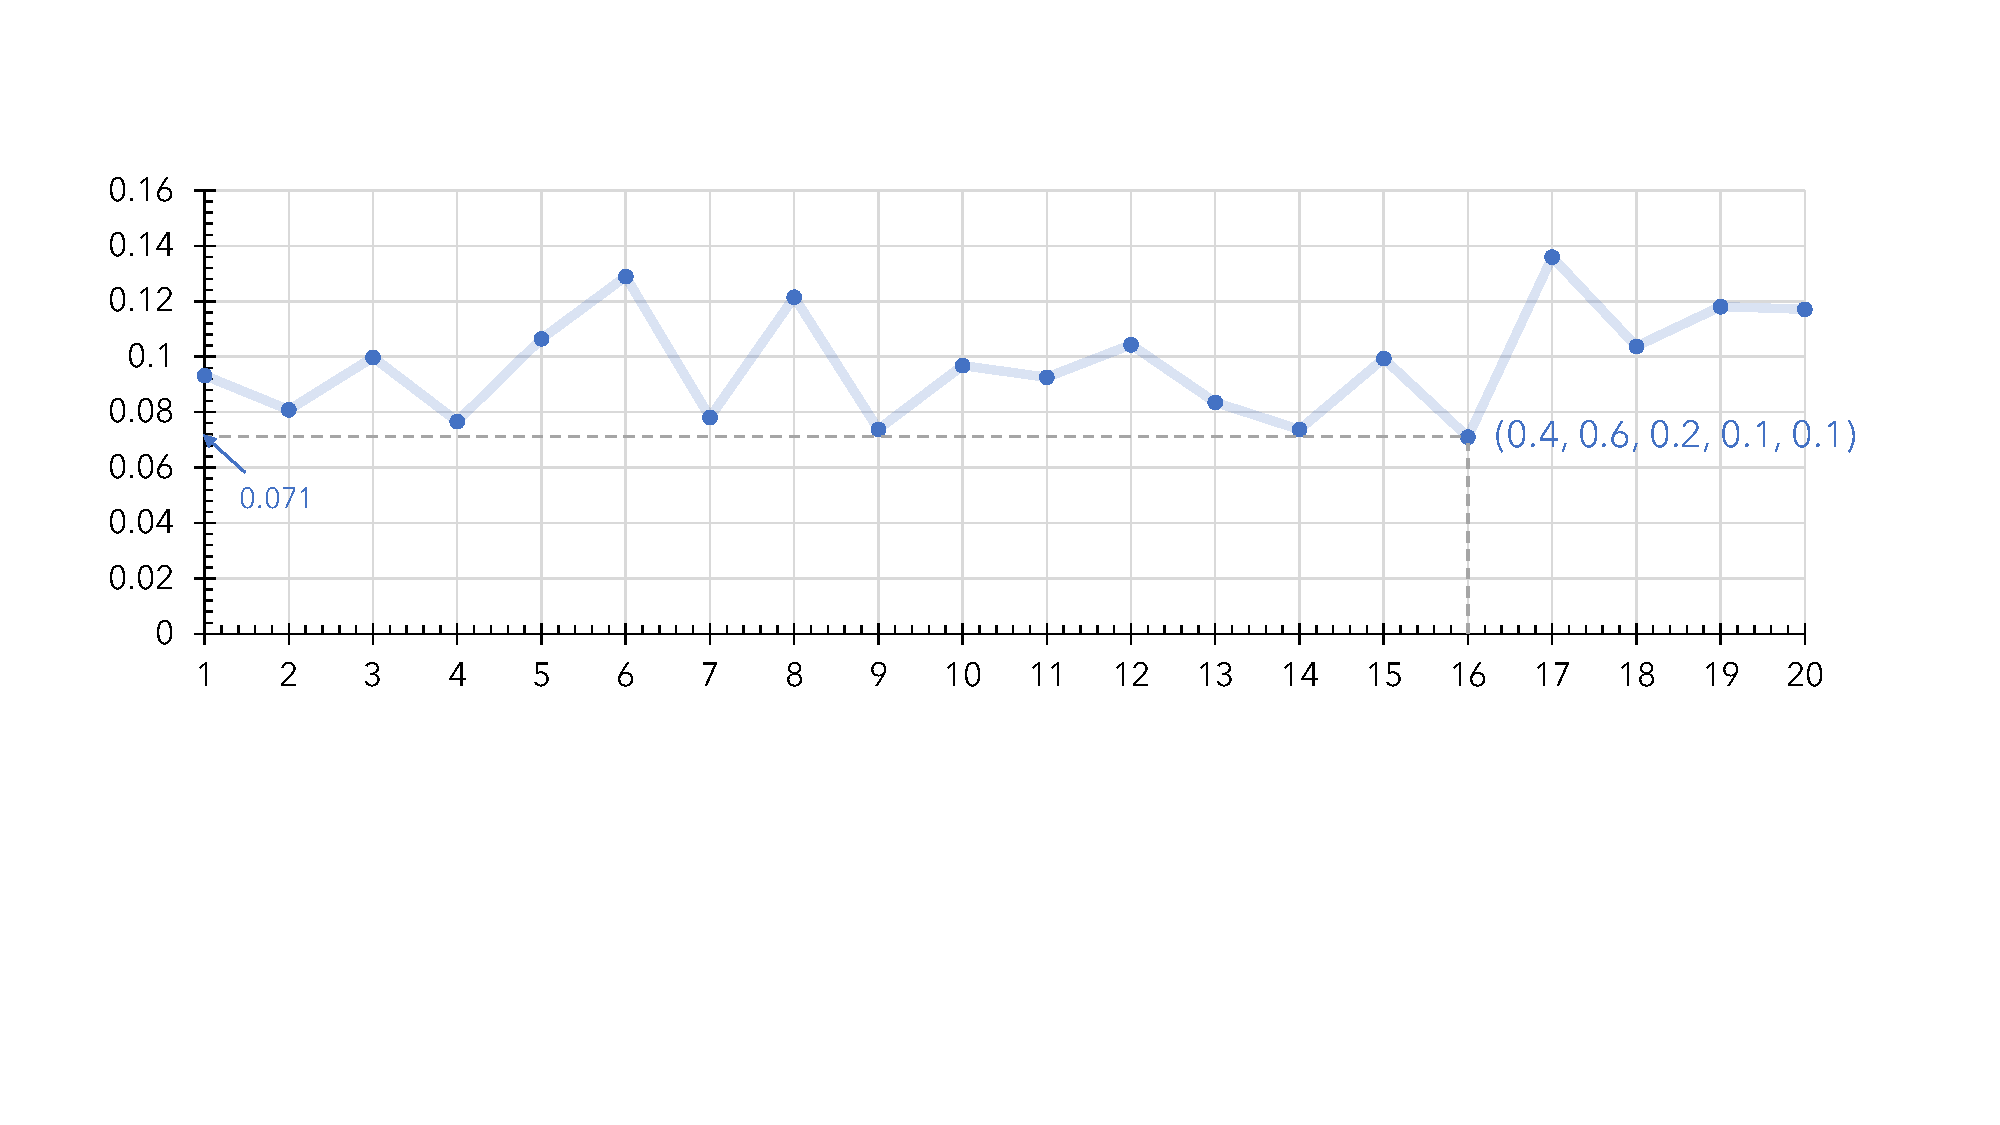
\includegraphics[width=.9\textwidth]{Lowest.pdf} 	% 图片相对位置
    \caption{$\mathtt{LowestError}$ of each possible weight}		% 图片标题 
    \label{fig:LowestError}							% 图片标签
\end{figure}

According to the training of the \textit{Greedy Algorithm}, there are 20 groups of weight coefficient combinations that meet the conditions. We calculate their $\mathtt{lowestError}$ respectively. As shown in \textbf{Figure \ref{fig:LowestError}}, the group with the lowest $\mathtt{lowestError}$ is selected as the final simulation result weight value $\hat{\beta}_i$.

\vspace{4pt}
\begin{itemize}
    \item \textbf{Simulation results and accuracy test}
\end{itemize}
According to our supervised observations of the model, the model can keep one decimal place for the weight value of each indicator. Finally, we put the last 5 matches into the test, and we can conclude that the model is valid. The model considers the regression formula for successful teamwork to be:
\begin{equation}
    S = 0.4x_1 + 0.6x_2 + 0.2x_3 + 0.1x_4 + 0.1x_5 + C
\end{equation}
i.e.
\begin{equation}\label{eq:regression_final}
    S = 0.4\gamma + 0.6\varphi + 0.2t_b + 0.1\sigma_y + 0.1\bar{x} + C
\end{equation}
Where the minimum error in the optimal weight $\mathtt{lowestError} = 0.071$, is valid for both data fitting and model regression. 
Through this model, we can score the team for each or teamwork for the entire season, and compare it with opponents, thus making the model adaptable.

From the regression equation \eqref{eq:regression_final} we get, we can have a general idea about the importance between the five indicators. 
\begin{itemize}
    \setlength{\parsep}{0ex} %段落间距
    \setlength{\topsep}{2ex} %列表到上下文的垂直距离
    \setlength{\itemsep}{1ex} %条目间距
    \item The most significant factor is the \textit{Distribution of contributions} as predicted, because it is linked with the final result directly. There is no doubt that a team, where every teammate contributes to the teamwork in his own position efficiently, has the strongest energy.
    \item  Next is the \textit{Coordination among players}, which is not difficult to understand.
    \item Then comes the \textit{flexibility}, \textit{tempo} and \textit{pressing}, which has relatively small weight, however can't be ignored.
\end{itemize}



\subsection{Discussion}
Depending on the model we constructed above, we can evaluate the success level of teamwork. The higher the value of performance indicators are, the higher the score $S$ is. However, in the model discussed above, we haven't taken the opponent into account. It's of great significance to clarify whether strategies are universally effective or dependent on opponents' counter-strategies. 

From the Evaluation Model we built in this section, the weights of different indicators are ascertained. It seems that as long as Huskies insists its strategy, which can be embodied by the five indicators, the score remains the same. However, this thought hasn't taken opponents' counter-strategies into consideration. We take the pressing as an example and draw the following \textbf{Figure \ref{fig:Comparison_pressing}}.
\begin{figure}[htbp]
    \centering
    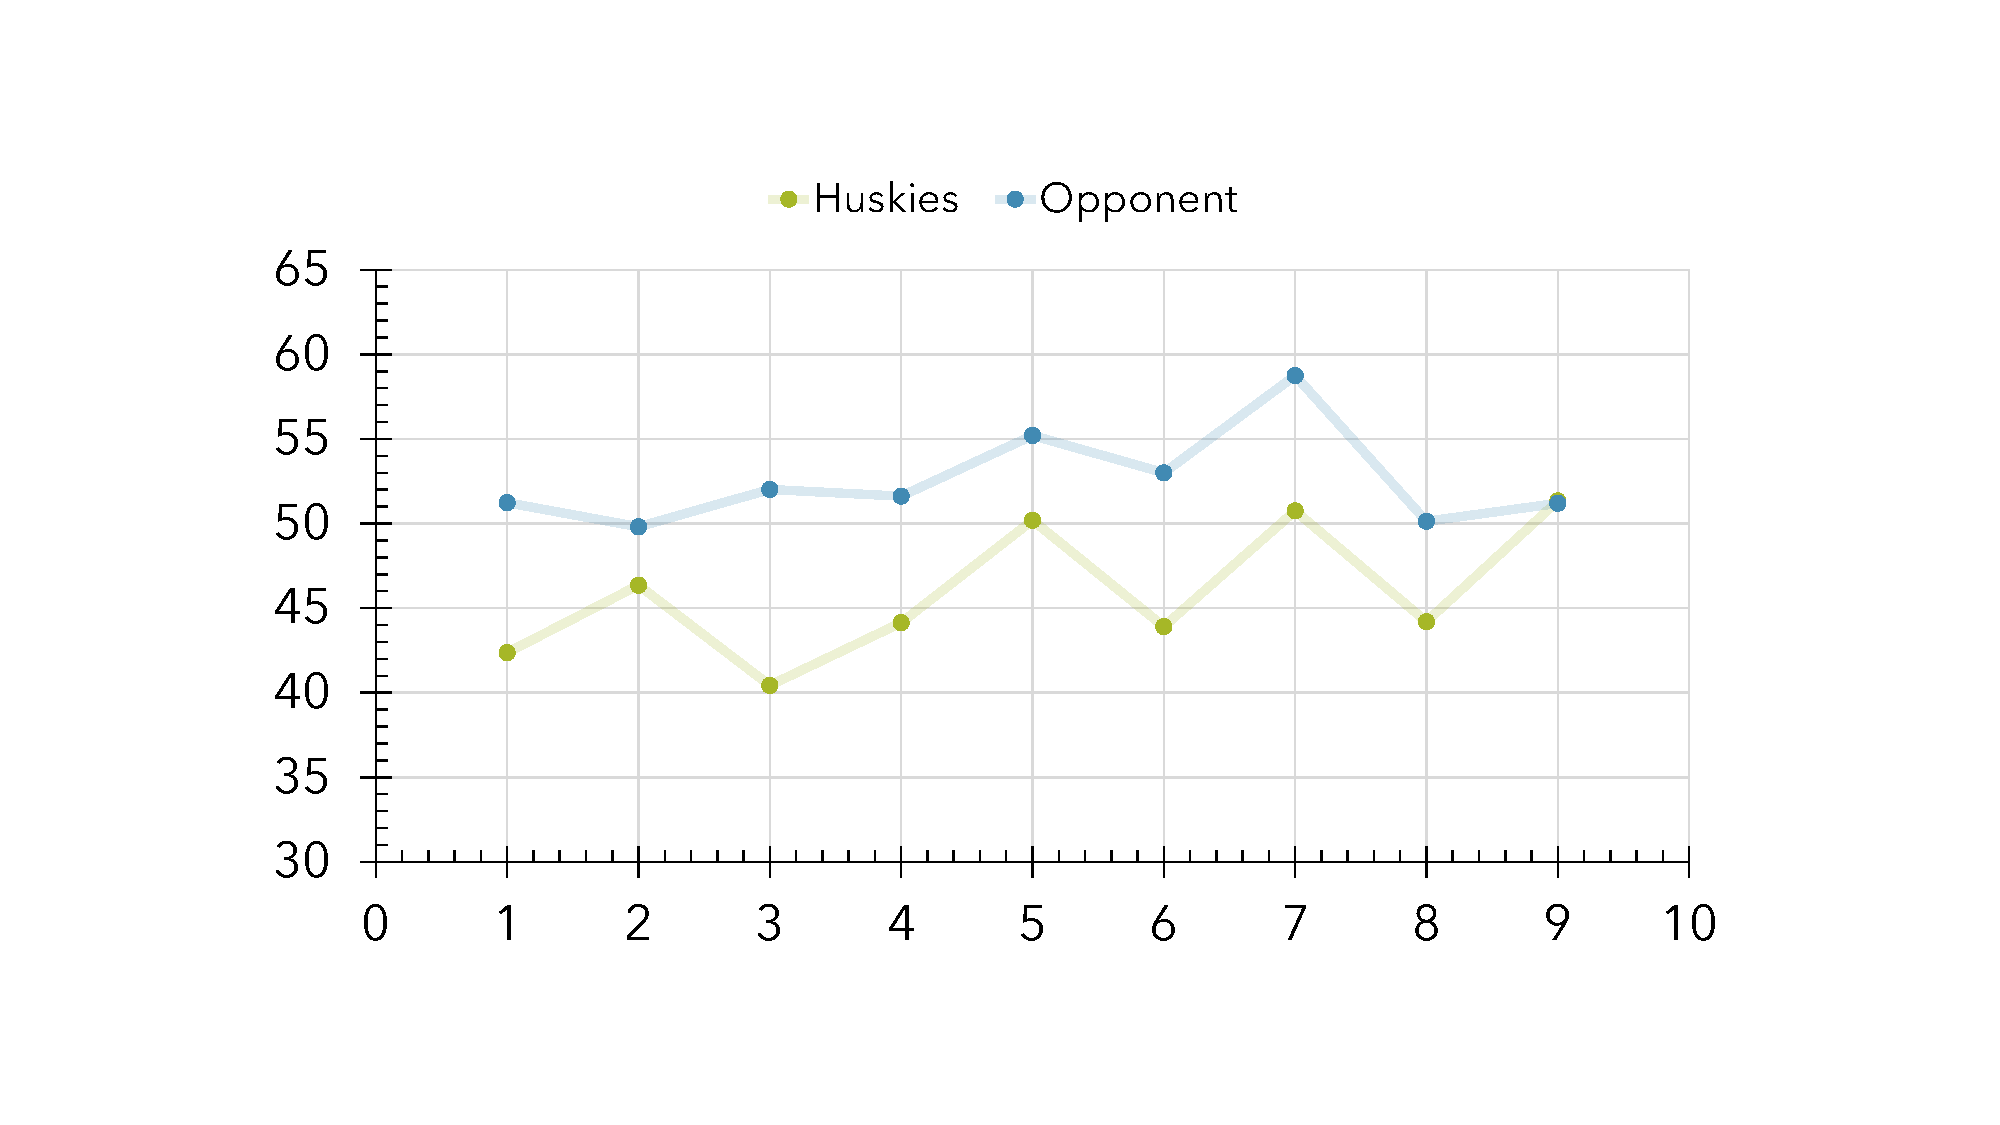
\includegraphics[width=.65\textwidth]{Comparison_pressing.pdf} 	% 图片相对位置
    \caption{Comparison of Pressing}		% 图片标题 
    \label{fig:Comparison_pressing}							% 图片标签
\end{figure}

From the \textit{Evaluation Model} we built in this section, the weights of different indicators are ascertained. It seems that as long as Huskies insists its strategy, which can be embodied by the five indicators, the score remains the same. However, this thought hasn't taken opponents' counter-strategies into consideration. For example, if the opponent's strategy makes the degree of pressing high, which means raise the $\bar{x}_{\mathrm{opponent}}$, the $\bar{x}_{\mathrm{Huskies}}$ of Huskies will decrease accordingly. That's to say, the value of indicators will be affected by opponents' strategy, thus influencing the score. Therefore, the strategy is not universally effective. Only by adjusting the strategy based on the opponents' strategy, trying to make the total score higher or repress the score of opponents, can one team make the likelihood to win higher. 





\section{\textsc{Task 3: }Advice on Improving Team Success}
\subsection{Structural Strategy Analysis}

After statistics of this season, the Huskies won \textbf{\textit{13}} matches, lost \textbf{\textit{15}} matches and tied \textbf{\textit{10}} matches in 38 games. For the team, the year-end data of this season is not ideal. In the next season, the team needs to make a huge change.

We have conducted a detailed analysis of the team data this season. In terms of \textit{team formation}, the formations used by different coaches are similar. From the data of 38 games, the main formation \textsf{4-3-3}, \textsf{4-4-2}, \textsf{5-3-2}, each game basically changes between these three formations. In general, we use \textsf{4-3-3} to represent the team's offense more, \textsf{4-4-2} to represent a conservative formation, and \textsf{5-3-2} to represent a more defensive formation. 

Below we analyze the five performance indicators mentioned in \textbf{\textsc{Task 2}} to determine the tactical system suitable for the current Huskies team. From the five indicators, we selected \textit{Coordination among players} (an indicator of teammate teamwork), \textit{Flexibility} (an indicator of offensive line diversity), and \textit{Pressing} (an indicator of team offense and defense status) to explore the three formations. Fitness for the team. We use indicators to determine the fitness of the three formations for the team separately.

\begin{table}[!htbp]
    \begin{center}
    \caption{Fitness of the three formations for the Huskies}
    \begin{tabular}{cccc}
        \toprule
        Formation  & Coordination & Flexibility & Pressing\\
        \midrule
        \textsf{4-3-3}	&5.1043	&32.42	&42.37\\
        \textsf{4-4-2}	&6.0104	&40.88	&43.58\\
        \textsf{5-3-2}	&7.5032	&23.50	&49.67\\
        \bottomrule
    \end{tabular}\label{tb:Fitness_formations}
    \end{center}
\end{table}

As is shown in \textbf{Table \ref{tb:Fitness_formations}}, the most suitable tactical formation for Huskies last season was \textsf{5-3-2}. 
\begin{itemize}
    \setlength{\parsep}{0ex} %段落间距
    \setlength{\topsep}{2ex} %列表到上下文的垂直距离
    \setlength{\itemsep}{1ex} %条目间距
    \item In this defense-based formation, the team's teamwork and offensive oppression are the highest, and it is the most effective strategy for now.
    \item However, this form of attack is not flexible enough, and the oppression is also very poor. It is almost oppressed by its opponents in its own half.
\end{itemize}  
So for Huskies at present, it is urgent to improve the offensive ability to win the match.

In summary, the Huskies need to give play to the characteristics of  \textit{good defense}, and strengthen the team's offensive capabilities. There are many classic football strategies, such as \textit{Tiki-Taka} (Barcelona), and \textit{Total Football} (Netherlands). Considering the actual situation of the Huskies, the most effective strategy is \textit{Defensive counterattack}.

\subsection{Comparison with \textit{Italy National Team}}
There are many teams that use defensive counterattacks in football, such as Real Madrid and Atlético Madrid. Here we choose Italy National Team which play the defensive counterattack to the extreme peak, and selected the classic battle - \textit{2012 European Cup semi-final} Italy v.s. Germany match data\upcite{7}, and compared with  average match data of the Huskies in this season.

\begin{figure}[htbp]
    \centering
    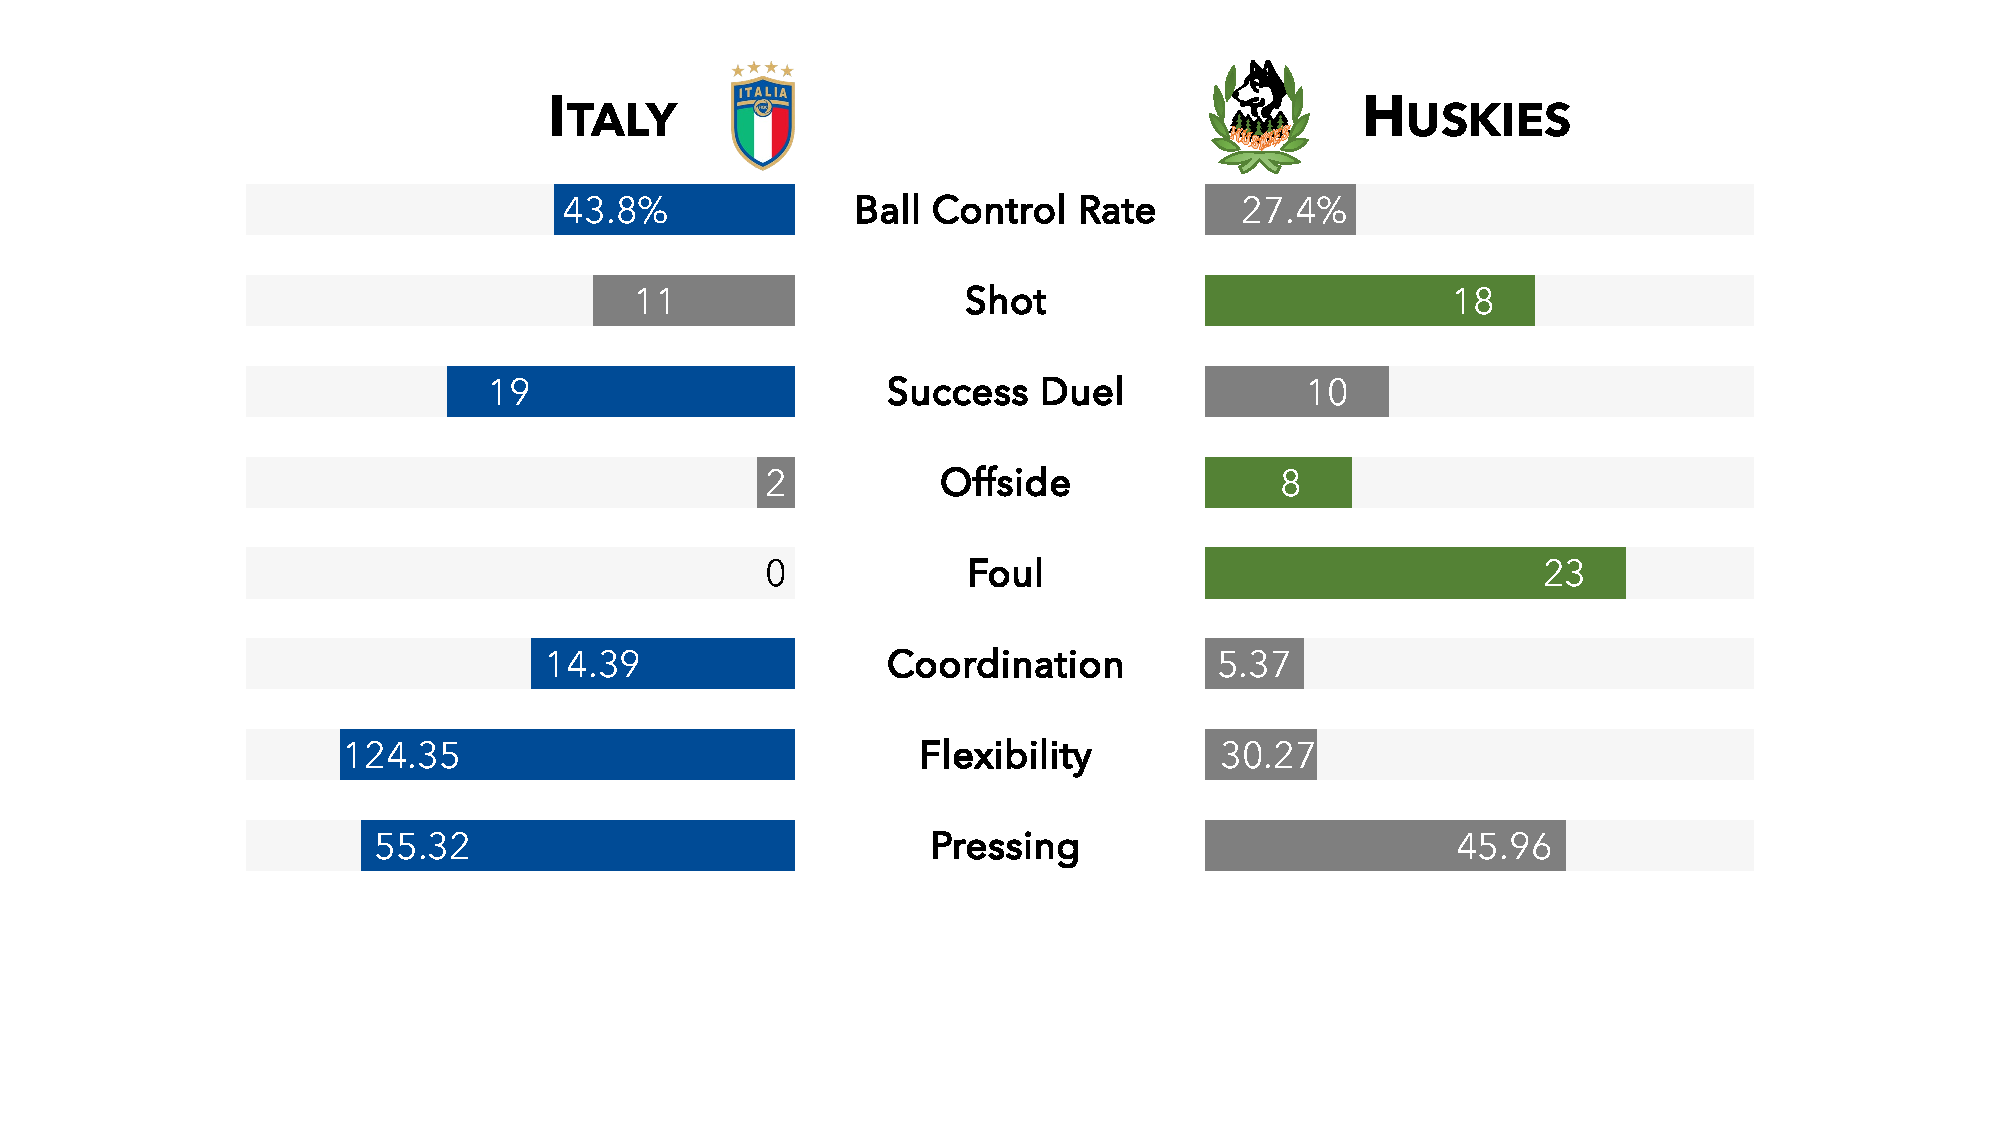
\includegraphics[width=0.8\textwidth]{Comparison_Italy.pdf} 	% 图片相对位置
    \caption{Comparison with Italy National Team}		% 图片标题 
    \label{fig:Comparison_Italy}							% 图片标签
\end{figure}

From the data in \textbf{Figure \ref{fig:Comparison_Italy}}, we can find that when facing  opponents that are stronger than themselves theoretically, such as Italy (FIFA World Ranking 14\textsuperscript{th}) v.s. Germany (FIFA World Ranking 1\textsuperscript{st}), whether it is in the case of \textit{Ball control rate}, or \textit{shot} is not dominant, still won the match 2-1. The winning experience of the Italy is the \textit{flexible change} of formation and the effective \textit{counterattack strategy}\upcite{8}.

Below we comment on Huskies' performance in this season. 
\begin{itemize}
    \setlength{\parsep}{0ex} %段落间距
    \setlength{\topsep}{2ex} %列表到上下文的垂直距离
    \setlength{\itemsep}{1ex} %条目间距
    \item The value of Coordination has been low, the team's cooperation lacking, resulting in a large number of \textit{Offside} and \textit{Foul}, unable to play a threatening cooperation.
    \item The number of Flexibility is not high enough. The team's offensive line is actually more simplistic. The tactics of the midfield straight out of the penalty zone cannot guarantee the goal rate and attack efficiency. The Huskies must choose to start from a wide open area.
    \item The Pressing value shows that the team is too conservative in defense. Most of the time it has been active in its own half, staying away from the opponent's goal, it is difficult to pose a threat, which reflects the lack of offensive organization ability of the team.
\end{itemize} 
 
In summary, in the change of next season, we should mainly consider the three indicators of \textit{Coordination}, \textit{Flexibility} and \textit{Pressing}, improve the diversification of the team's offensive methods, and defensive counterattack with efficient and threatening organizations.

\subsection{Advise on next Season}
After analyzing our team's network and strategy this season, in order to achieve successful teamwork and better team performance next season, the changes that the team needs to make now are:
\begin{enumerate}[\bfseries \text{Change} 1:]
    \item \textit{Adjusted the formation to a more flexible formation}
    
    From the data of this season, we can see that the team is good at \textit{defending} this work, but the cooperation is not enough. So we will choose \textsf{4-1-3-2} as the team's main formation next season. It is flexible and can be evolved into \textsf{5-3-2} and \textsf{4-3-3}.
    \item \textit{Highlight the importance of core players}
    
    In team cooperation, we must make the best use of every character in the team to maximize their value. From the situation of last season, \texttt{M2} and \texttt{F1}, \texttt{F2} should be the core points of the offense. When \texttt{M2} holds the ball, it should The deformed formation is \textsf{5-3-2} or \textsf{4-3-3} to protect \texttt{M2} players from holding the ball. \texttt{F1} and \texttt{F2} should find more neutral and running positions in the frontcourt to respond to the midfield pass.
    \item \textit{Coherence of possession and defense}
    
    The key to the \textsf{4-1-3-2} formation of ball control is not multi-ball control, but to control the ball on the center line of the court as far as possible, where Advance attack, retreat defend.
\end{enumerate}

\begin{figure}[htbp]
    \centering
    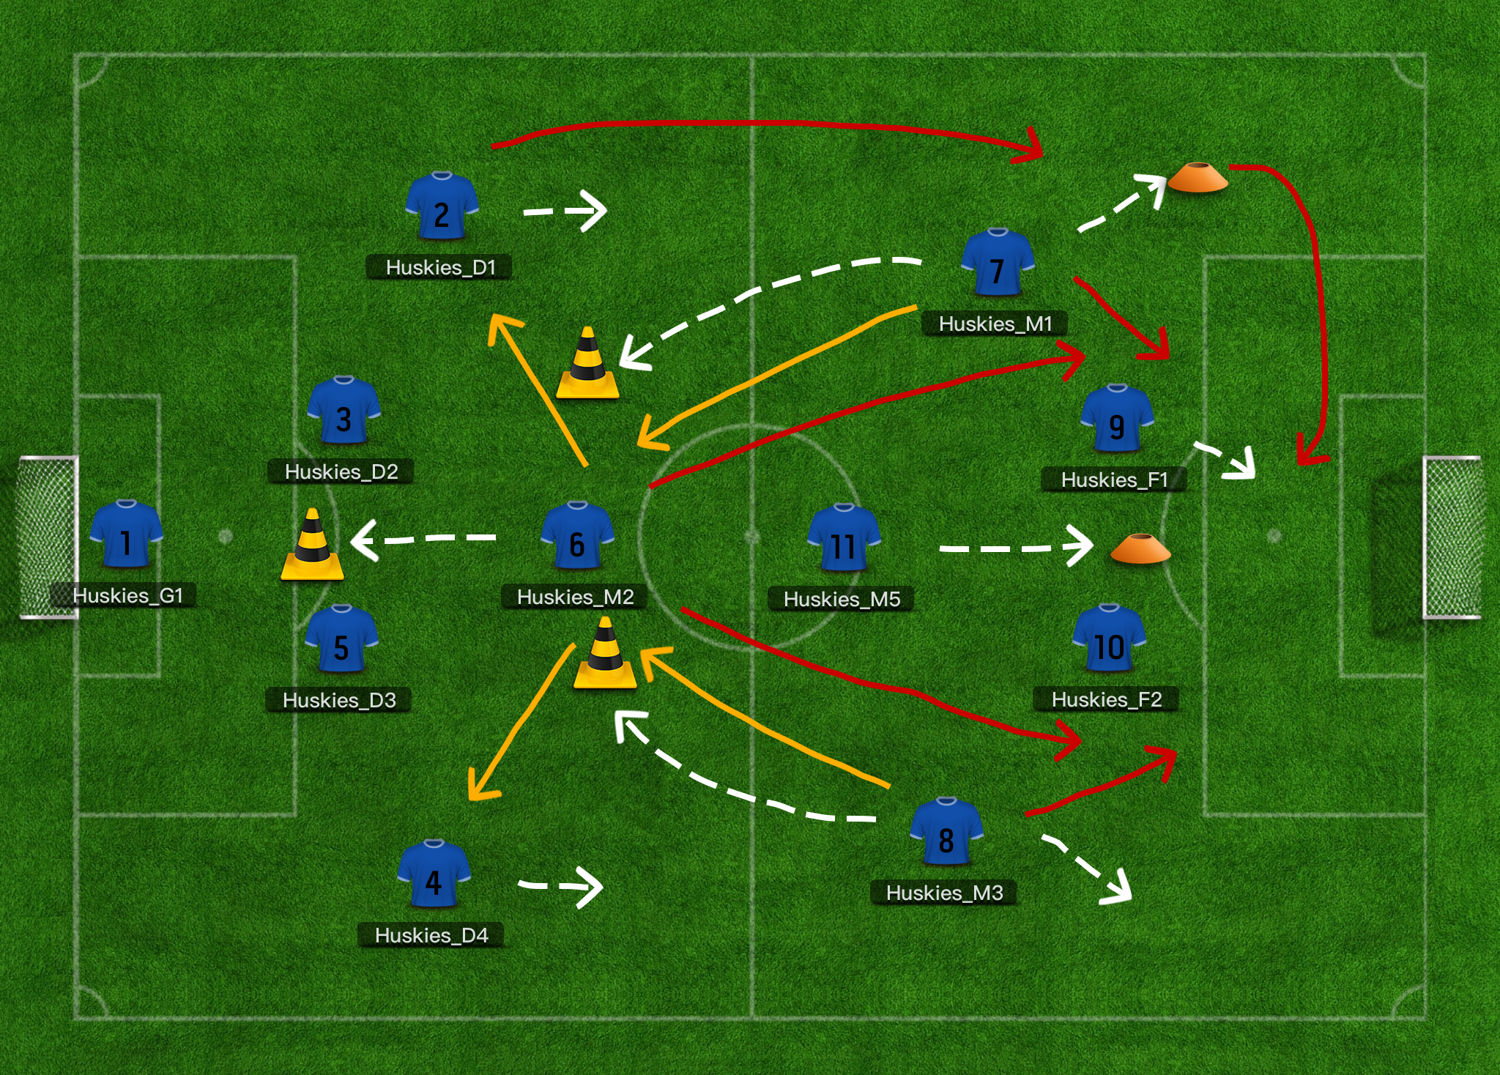
\includegraphics[width=.75\textwidth]{task3_formation.png} 	% 图片相对位置
    \caption{A schematic diagram of \textit{Defensive counterattack}}		% 图片标题 
    \label{fig:task3_formation}							% 图片标签
\end{figure}

As is shown in \textbf{Figure \ref{fig:task3_formation}}, the \textit{white dotted line} represents the player's moving route. Adapt to the player's moving route, the \textsf{4-1-3-2} formation can be changed to \textsf{5-3-2}, \textsf{4-3-3}, \textsf{4-3-1-2} and other formations according to the situation on the court or the opponent's strategy. The \textit{red solid line} represents the team's pass line when attacking. The initiator of the attack is usually organized by \texttt{M2}. At this time, \texttt{M1} and \texttt{M3} need to back up and protect \texttt{M2} to control the ball, or insert to create an offensive opportunity. The \textit{yellow solid line} represents the passing route when defensive is needed or when there is no good offensive neutral, increases the ball control rate, and stabilizes the ball right near the center axis. The \textit{yellow Warning sign barrel} represents the position that the returning player needs to return. The \textit{orange flag bucket} represents where the offensive player can launch a threatening attack.

\section{\textsc{Task 4}: How to Design more Effective Teams}
\subsection{Generalization of our Model}\label{sec7.1}
In a gesture to design more effective teams, we can generalize our model to other practical teamwork. It is of great significance to understanding the complex set of factors that make some groups perform better than others. In this chapter, we make several analogies to the indicators we used in the team sport model. 
\vspace{4pt}
\begin{itemize}
    \item \textbf{Coordination among teammates}
\end{itemize}

\begin{figure}[htbp]
    \centering
    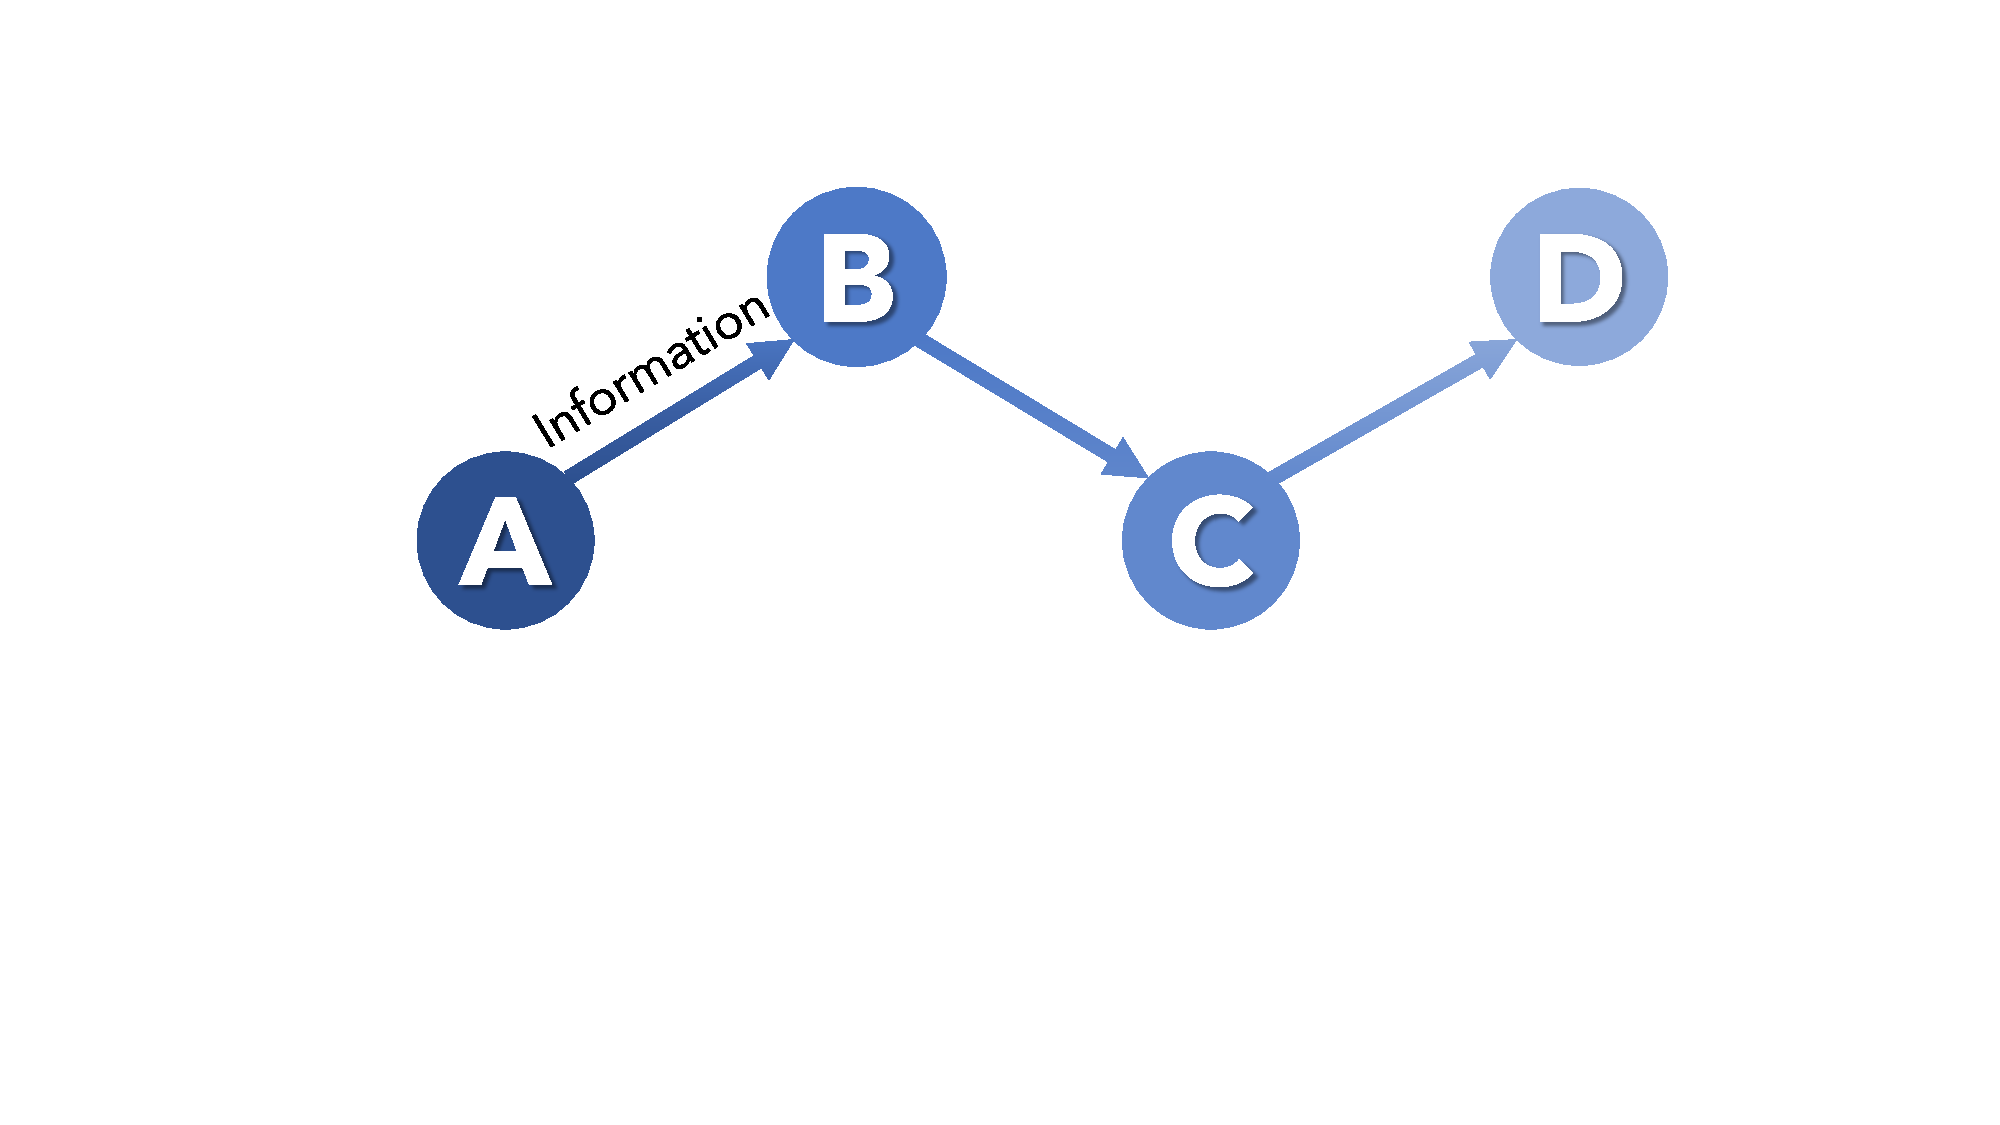
\includegraphics[width=.35\textwidth]{Coordination.pdf} 	% 图片相对位置
    \caption{Coordination among teammates}		% 图片标题 
    \label{fig:Coordination}							% 图片标签
\end{figure}

Similar to the connection between players, the closeness of connection between colleagues is also an important indicator of teamwork. In terms of the coordination among teammates, we can use the informational passing distance $d$ to quantify this parameter, which means the number of the teammates the instruction get through when it is being passed between the team. Just as \textbf{Figure \ref{fig:Coordination}} shows.


The distance between \textit{A} and \textit{B} is 1, while \textit{A} is 3 away from \textit{C}. Then we can get a similar network matrix like passing matrix. In this way, \textit{cluster coefficient} can also be used here to quantify the coordination among teammates. 


\begin{itemize}
    \item \textbf{Distribution of contributions}
\end{itemize}

For teamwork, a reasonable and appropriate division of labor is also an important indicator of cooperation efficiency. In teamwork, everyone should perform his or her own duties to promote strengths and avoid weaknesses.

Unlike football games where contribution can be easily divided into two aspects, offence and defense, the contribution in other teamwork is more complex. Each teammate has his or her own position and performance evaluation criteria. Therefore, for people in different position the quantification rules vary from each other. 

\vspace{4pt}
\begin{itemize}
    \item \textbf{Flexibility}
\end{itemize}

In teamwork, it is inevitable that we will encounter difficulties and setbacks. At this time, we need to be flexible to make changes and try boldly. The Huskies performed poorly with the \textsf{4-3-3} formation in the 9th match, but later quickly changed to reverse the situation. 

With reference to the variety of attack strategy, we can make an analogy to the standard deviation of $x$-coordinate value where each passing event happens. For each team, the final target may be unique, but the plan isn't limited. Consequently, we can use the standard deviation of the number of people dispatched to different plans to quantify the flexibility. 


\subsection{Other Aspects}\label{sec7.2}
Considering the complexity in other practical teamwork, we need to take more aspects into consideration to develop generalized models of team performance. 

\begin{itemize}
    \item \textbf{Ideal leadership style}
\end{itemize}

Each team has one leader, who help leverage the skills of all their teammates and make overall plan. A good leader can make teamwork more efficient. Therefore, it is important to evaluate the leadership and leadership style. 


There are many leadership styles. A leader will lead several people directly or indirectly. We can use the distance to quantify the leader's leadership intensity $I$ as the formula shows:
\begin{equation}
    l=\sum_{i=1}^{N}\frac{1}{d_N}.
\end{equation}
Where $N$ is  the total number of people the leader leads, and $d_N$ is the distance between the person and the leader.
The management scientists make out a leadership intensity standard\upcite{9}. When this leadership strength is exceeded, the leader will be \textit{tired} in the management process. On the contrary, when the management intensity is too low, the managerial talents are not fully applied, which causes the idleness of human capital. Therefore, building a leadership model and choosing the ideal leadership style also play a dominant role. 


\vspace{4pt}
\begin{itemize}
    \item \textbf{Effective coordination over time}
\end{itemize}

The effective coordination can be expressed as follow: 
\begin{equation}
    E=\frac{\displaystyle\sum_{i=1}^N t_{\mathrm{work}}}{t_{\mathrm{total}}}.
\end{equation}
Where $t_{\mathrm{work}}$ is the total time one person working, and $t_{\mathrm{total}}$ is  the total duration of the entire cooperation.

For example in football game, as one player steals the ball from an opponent, another player is poised for offense. Their total working time is definitely larger than the time the whole event takes, which means they have higher effectivity. In comparison, we can also use this method to quantify the effective coordination over time. 





\section{Analysis on Model's Sensitivity}
\subsection{Evaluation Model sensitivity to \textit{Draw} situations}
When studying the Evaluation model in \textbf{\textsc{Task 2}}, we dealt with the situation when the two teams were tied by  absolute difference. When the difference in absolute value of evaluation score $S$ is less than 1, we regard this situation as the indicator passed. 
Next, we will study the influence of the constraints on the \textit{difference between the scores} of the two teams (error limit) on the \textit{weight value} $\beta_i$ in the model.

We let ${\left| S_1-S_2 \right| < \varepsilon}$, where error limit $\varepsilon \in [0,2]$. We substitute the error limit into the model algorithm, calculate the value of each weight $\beta_i$ under different error limit $\varepsilon$, and calculate the $\mathtt{lowestError}$. Finally, we draw a visual smooth curve like \textbf{Figure \ref{fig:sensitive_analysis1}}.
\begin{figure}[htbp]
    \centering
    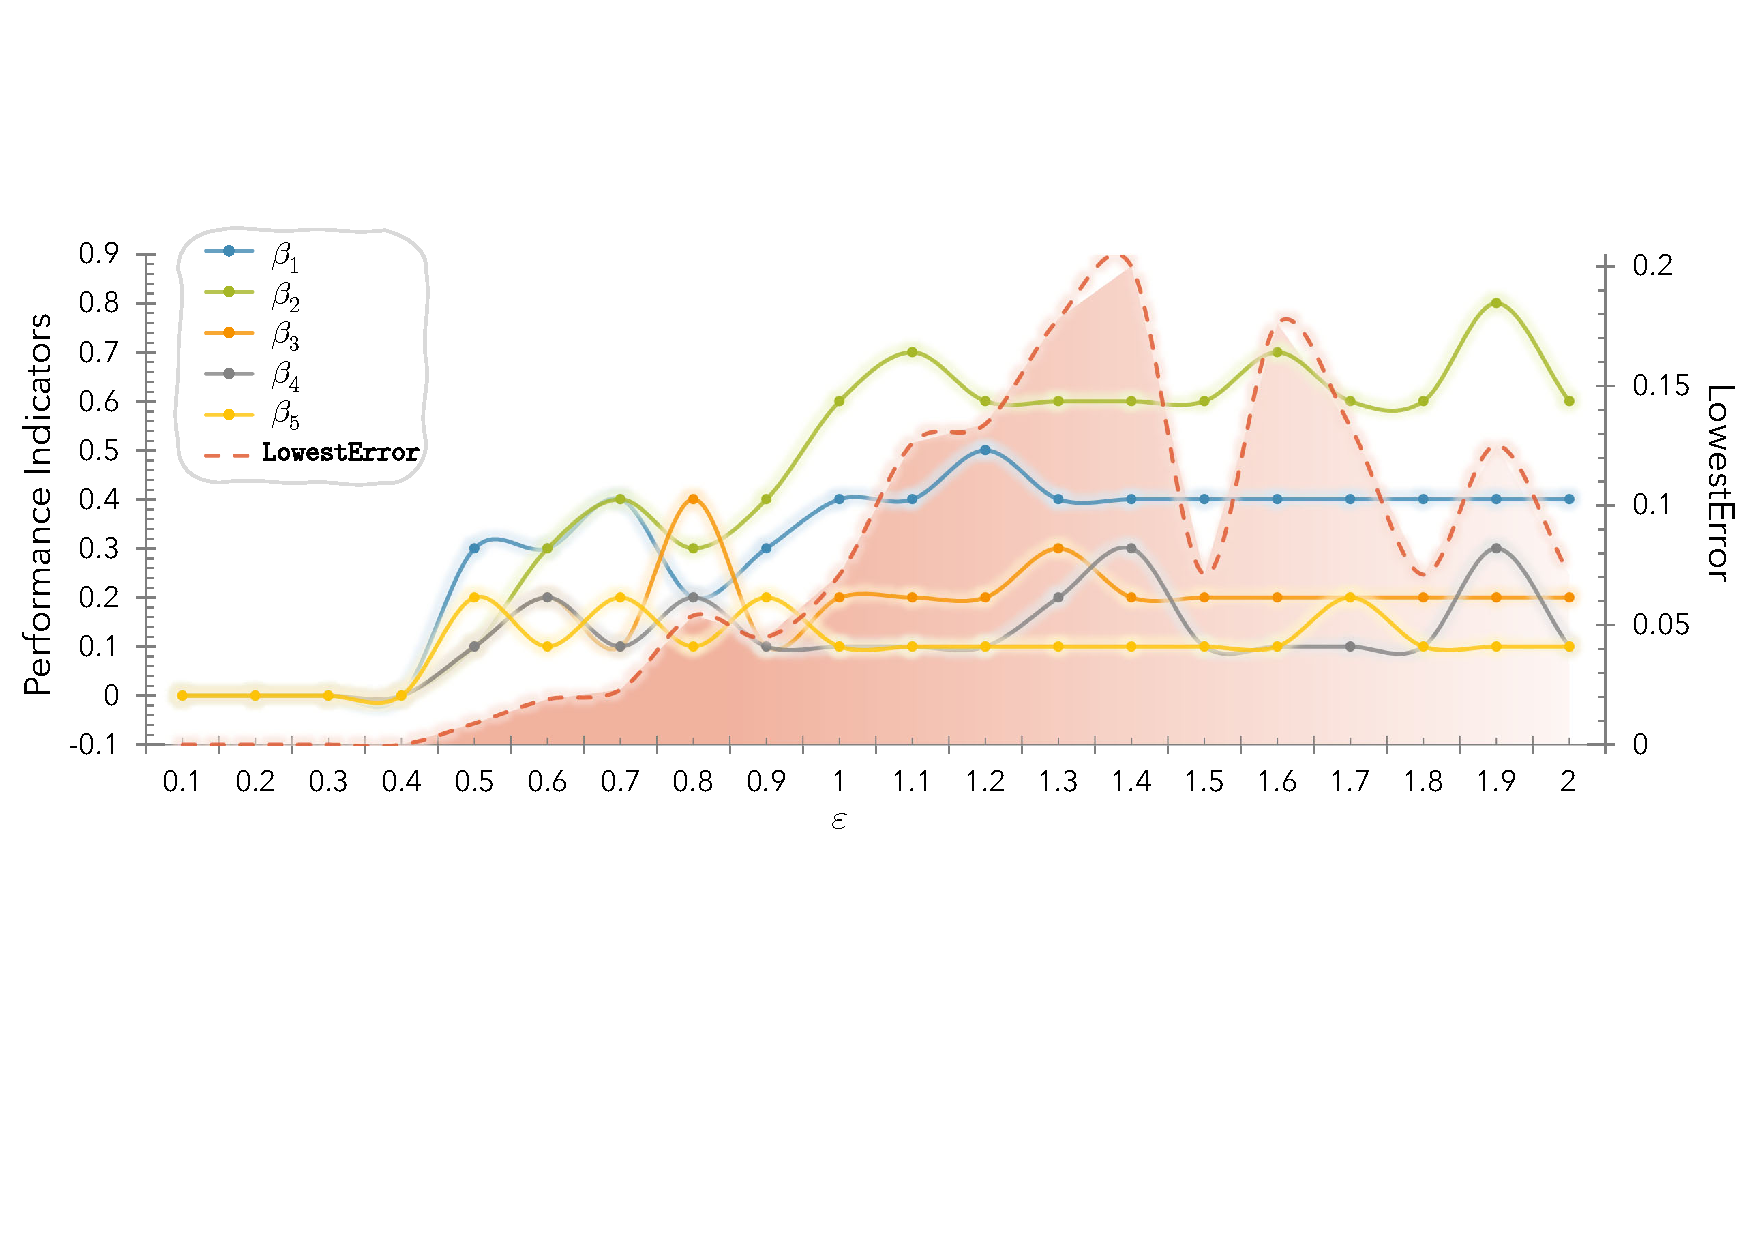
\includegraphics[width=1.0\textwidth]{sensitive_analysis1.pdf} 	% 图片相对位置
    \caption{Five performance indicators and $\mathtt{lowestError}$ with different error limit $\varepsilon$}		% 图片标题 
    \label{fig:sensitive_analysis1}							% 图片标签
\end{figure}

In \textbf{Figure \ref{fig:sensitive_analysis1}}, we can see that when $\varepsilon <1$, the $\mathtt{lowestError}$ has been kept at a low level. However, at this time the weights of the five indicators of the model have been in a chaotic state and cannot reflect the reality and the importance of the indicators. 
When $\varepsilon> 1$, the weight of each indicator is relatively stable. At this time, we must also consider the value of $\mathtt{lowestError}$, and the deviation should not be too large. It can be seen that when $\varepsilon = 1, 1.5, 1.8$, it is more reasonable as a tie. So our model is more sensitive to the situation of a draw.

\subsection{Analysis on performance indicator \textit{Tempo}}
In \textbf{Task 2}, the quantitative indicator for reflecting the {Tempo} on the football field is the time it takes for a player to pass 50 goals. Here we consider whether the time when players pass 10, 30, 50, 70, 90 balls can appropriately reflect the changing rhythm on the court. In order to make the time of different foot counts analyzable, we choose the same game time to prevent the situation where tempo cannot be compared due to different time intervals.

After our analysis of the data, we chose 46 s - 1305 s in the first half of the match. And we removed the \textit{10-pass} and \textit{90-pass} time because their time is too short or too long to analyze the sensitivity.  Through calculation, we obtain the time curve of  ball passing time per 30, 50, 70 passes during this period.
\begin{figure}[htbp]
    \centering
    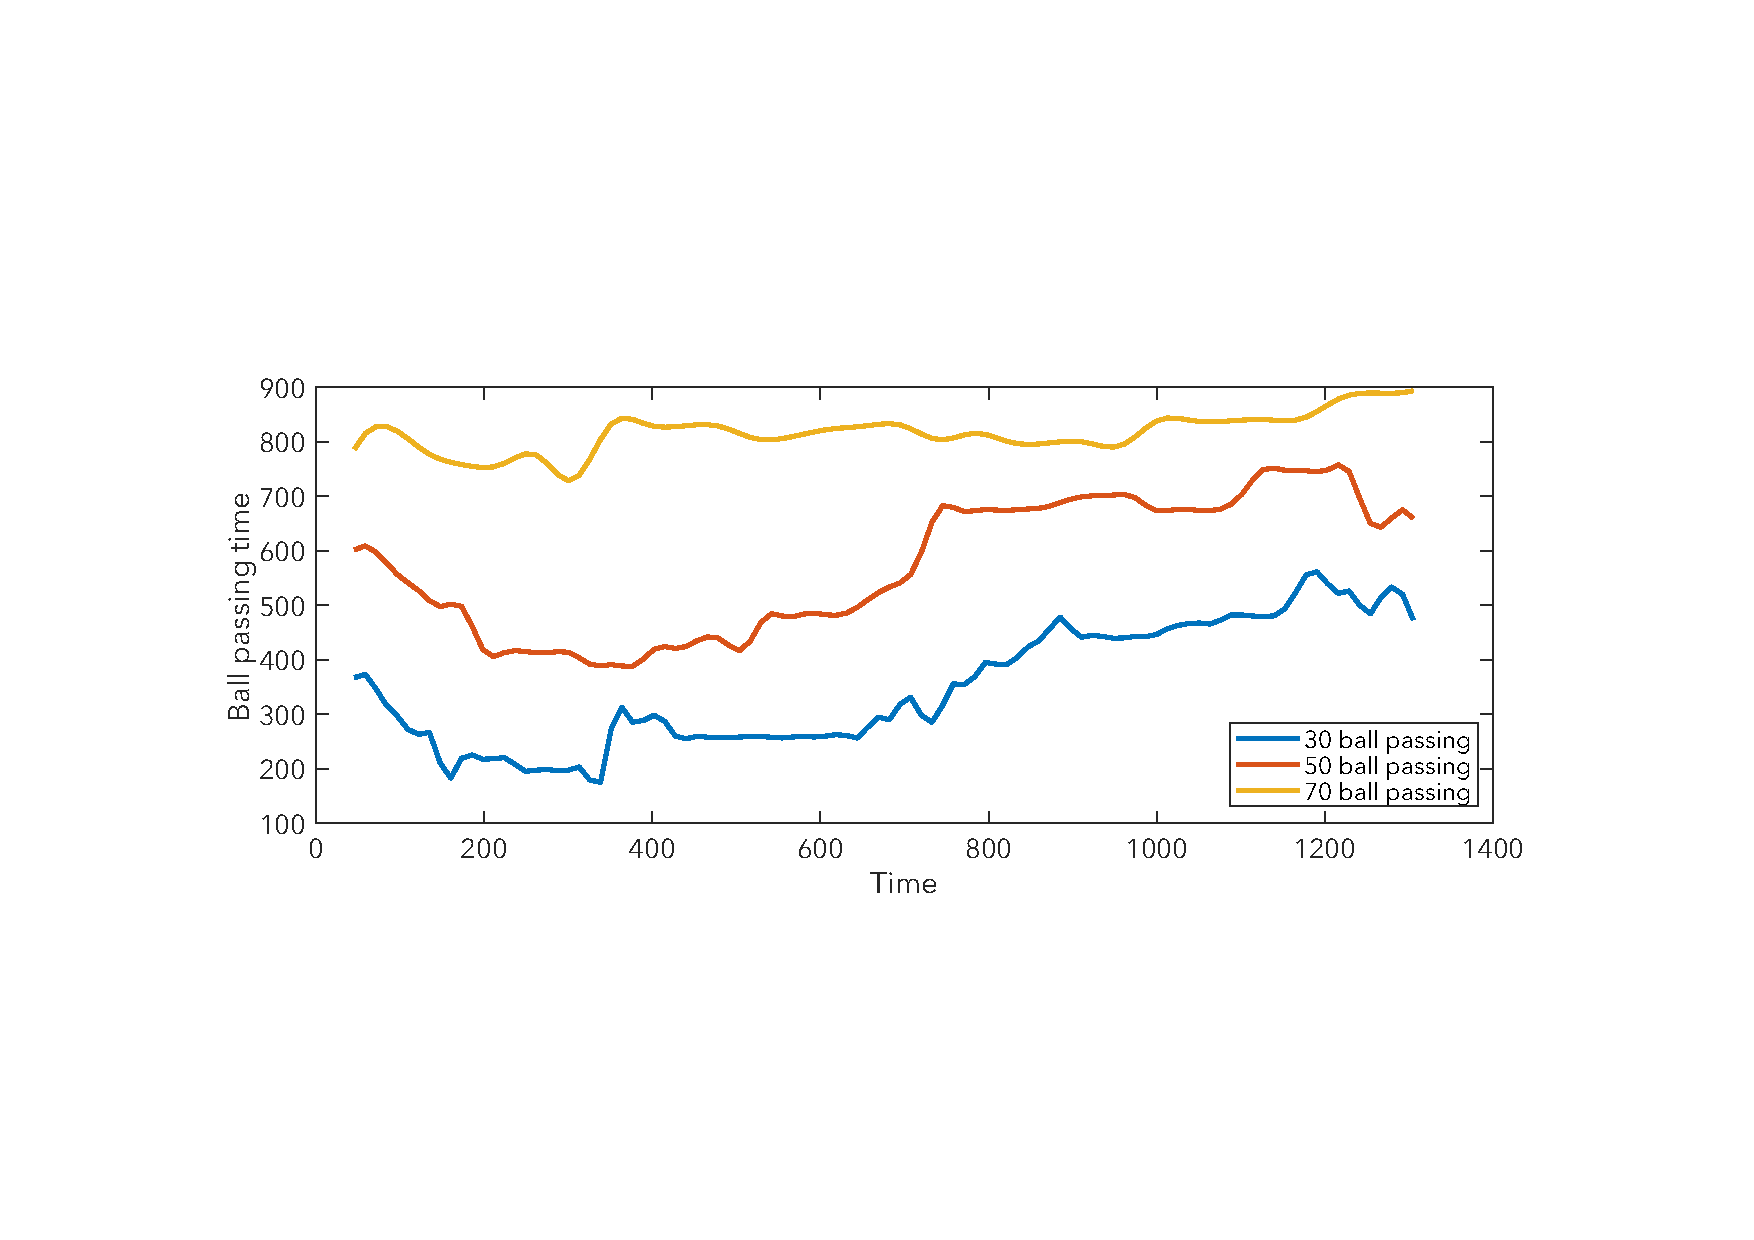
\includegraphics[width=.90\textwidth]{sensitive_analysis2.pdf} 	% 图片相对位置
    \caption{Ball passing time per 30, 50, 70 passes}		% 图片标题 
    \label{fig:sensitive_analysis2}							% 图片标签
\end{figure}

As can be seen from \textbf{Figure \ref{fig:sensitive_analysis2}}, when calculating the \textit{30-pass time}, the curve shows more jagged parts, that is, the tempo on the football field has a clear turning point. This is well understood according to the actual situation of the football field. When dividing the passing time, the tempo displayed on the court will not change much (i.e., it is difficult to change the defensive or offensive rhythm within 30 feet). When calculating the \textit{70-pass time}, there is almost no change in tempo on the field, which is obviously not reasonable. The tempo indicator in our model is sensitive to the number of passes hence. This is why the \textit{50-pass time} is the most scientific and reasonable to calculate tempo.


\section{Strengths and Weaknesses}
\subsection{Strengths}
\begin{itemize}
    \item The selection of the network parameters of the passing network is scientific and reasonable. The network model is highly applicable and can reflect the characteristics of various aspects of the team and the evaluation scale.
    \item The evaluation model also introduces the opponent into the evaluation system. In order to be able to compare against the Huskies team, the weight coefficients of the five indicators are returned to be more scientific and reasonable.
    \item Our model analyzes the Huskies team's data thoroughly, finds more effective strategies for the team, proposes constructive changes, and visualizes our strategies.
\end{itemize}
\subsection{Weaknesses}
\begin{itemize}
    \item Our model did not have enough analysis and processing for the eventsubtype part, and did not take out each team member for individual analysis.
    \item The indicators of the popularization model cannot be quantified, resulting in a low persuasibility of the model.
  \end{itemize}


% \section{Model Promotion}
% The model can be extended to many industries, such as the courier industry, the medical industry, the retail industry.
% Take the courier industry as an example, we can compare a courier point to a charging station. Courier service range corresponds to the mileage of the electric car after charging, while the average delivery time corresponds to the average waiting time for electric car charging. Moreover, the demand for expressing delivery is very different in cities, suburbs and villages. Therefore, it is completely possible to use the charging station model to distribute the courier points.

% \section{Conclusion}
% \begin{itemize}
%     \item In the future, it is very likely that among the majority of countries, electric vehicles will be completely popularized. Besides, the stagnation of the rest countries could be attributed to their own geographical reasons, such as Indonesia, Venice and other countries or regions.
% \item The main influencing factors which trigger different modes of network growth contain the density of population, the distribution of wealth, the strength of science and technology and cost. Besides, different factors may cause different effects.
% \item The cost has a great influence on the development of the charging station network, while the population density has only a slight impact.
% \end{itemize}



% 参考文献,此处以 MLA 引用格式为例
\clearpage
\begin{thebibliography}{99}
    \bibitem{1} Leighton, F. Thomson. \emph{Introduction to parallel algorithms and architectures: array, trees, hypercubes}. 2014.
    \bibitem{2} Clemente, Filipe Manuel, et al. "General network analysis of national soccer teams in FIFA World Cup 2014." \emph{International Journal of Performance Analysis in Sport} 15.1 (2015): 80-96.
    \bibitem{3} Dijkstra, Edsger Wybe. "A Note on Two Problems in Connexion With Graphs." \emph{Numerische Mathematik} 1(1959):269-271.
    \bibitem{4} Ahnert, Sebastian E., et al. "Ensemble approach to the analysis of weighted networks.." \emph{Physical Review E} 76.1 (2007).
    \bibitem{5} Wong, J. A. Hartiganm. A. . "Algorithm AS 136: A K-Means Clustering Algorithm." \emph{Journal of the Royal Statistical Society. Series C (Applied Statistics)} 28.1(1979):100-108.
    \bibitem{6} Buldu, J. M., et al. "Defining a historic football team: Using Network Science to analyze Guardiola’s F.C. Barcelona." \emph{Scientific Reports} 9.1 (2019): 1-14.
    \bibitem{7} \emph{Balotelli sends Italy past Germany}. (2012). Retrieved December 10, 2014, from\url{https://www.uefa.com/uefaeuro/season=2012/matches/round=15174/match=2003379/index.html}
    \bibitem{8} Sigari, Mohamad Hoseyn, et al. "Counterattack detection in broadcast soccer videos using camera motion estimation." \emph{international symposium on artificial intelligence} (2015): 101-106.
    \bibitem{9} Abdelmahmoud Hassan Elsheikh. \emph{Effect of Leadership Intensity on Integrating Some Formal and Informal Organizational Efforts for Community Development in Khartoum Province}. 2016.
\end{thebibliography}
% \includepdf[pages={1,2}]{Memo.pdf} 
\begin{subappendices}  % 附录环境

    \section{Appendix: Code}
    \noindent \textsc{Task 1} - \textbf{matrix.m}
\lstinputlisting[language=matlab]{./code/matrix.m}

\noindent \textsc{Task 1} - \textbf{passingtime.m}
\lstinputlisting[language=matlab]{./code/passingtime.m}

\noindent \textsc{Task 2} - \textbf{AdversarialRegression.py}
\lstinputlisting[language=python]{./code/AdversarialRegression.py}
       
    \end{subappendices}
\end{document}  % 结束